\documentclass[12pt]{article}

\PassOptionsToPackage{a6paper, landscape, margin=5mm}{geometry}
\PassOptionsToPackage{table}{xcolor}

\usepackage{
	geometry,
	multicol,
	lmodern,
	newtxtext,
	newtxmath,
	newtxtt,
	parskip,
	ragged2e,
	multirow,
	graphicx,
	subcaption,
	xcolor,
	lastpage
}

\newcommand{\foreign}[1]{\textit{#1}}

\def\True{\mathtt{True}}
\def\False{\mathtt{False}}

\newcommand{\slide}[3]{
	\raisebox{.5em}{\bfseries\Large #1}
	\hfill
	
\includegraphics[height=10mm]{img/logo-math}
	
\includegraphics[height=10mm]{img/logo-classic}
	\vspace{.25em} \hrule
	\vfill

	\begin{center}
		#2
	\end{center}

	\vfill
	\hrule
	{#3}
	\hfill
	\thepage\ / \pageref{LastPage}
	\clearpage
}

\newcommand{\titleslide}[1]{
	\slide{\normalfont Sidang Tugas Akhir}{#1}{\theYear}
}

\newcommand{\outline}[1]{
	\slide{Outline}{
		\begin{multicols}{2}
			{\ifnum#1=1\bfseries\fi Permasalahan}

			{\ifnum#1=2\bfseries\fi \foreign{Distance Similarity Matrix}}

			{\ifnum#1=3\bfseries\fi Formulasi Algoritma}

			{\ifnum#1=4\bfseries\fi Evaluasi Algoritma}

			{\ifnum#1=5\bfseries\fi Hasil dan Pembahasan}

			{\ifnum#1=6\bfseries\fi Kesimpulan}
		\end{multicols}
	}{}
}


\newcommand{\titleBahasa}{Menentukan Dimensi Metrik Menggunakan \foreign{Satisfiability Modulo Theories}}

\newcommand{\titleEnglish}{Determining Metric Dimension with Satisfiability Modulo Theories}

\newcommand{\theAuthor}{Fikri Yudhistira Ajiwijaya}
\newcommand{\theAuthorId}{5002211165}

\newcommand{\supervisor}{Muhammad Syifa'ul Mufid S.Si, M.Si, Ph.D}
\newcommand{\supervisorId}{198909112014041001}

\newcommand{\examinerOne}{Dr. Dieky Adzkiya, S.Si, M.Si}
\newcommand{\examinerOneId}{198305172008121003}

\newcommand{\examinerTwo}{Soleha, S.Si, M.Si}
\newcommand{\examinerTwoId}{198301072006042001}

\newcommand{\examinerThree}{Muhammad Luthfi Shahab, S.Si, M.Si, Ph.D}
\newcommand{\examinerThreeId}{199503312018031001}

\newcommand{\programChair}{Dr. Tahiyatul Asfihani, S.Si, M.Si}
\newcommand{\programChairId}{198707282014042001}
\newcommand{\programChairTitle}{Kepala Proram Studi Sarjana}

\newcommand{\documentName}{Tugas Akhir}
\newcommand{\degreeName}{Sarjana Matematika}
\newcommand{\programName}{Program Studi S-1 Matematika}
\newcommand{\departmentName}{Departemen Matematika}
\newcommand{\facultyName}{Fakultas Sains dan Analitika Data}
\newcommand{\facultyNameAbbreviated}{FSAD}
\newcommand{\campusName}{Institut Teknologi Sepuluh Nopember}
\newcommand{\campusNameAbbreviated}{ITS}

\newcommand{\theCity}{Surabaya}
\newcommand{\theDay}{\the\day}
\newcommand{\theMonth}{\bulan{\the\month}}
\newcommand{\theYear}{\the\year}

\title{\titleBahasa}
\author{https://github.com/wijayarakhmat98/metric-dimension}


\begin{document}

\titleslide{
	\textbf{\Large \titleBahasa}

	\vfill

	\textbf{\theAuthor} \\
	NRP. \theAuthorId

	\textbf{\supervisor} \\
	NIP. \supervisorId

	\vfill

	\departmentNameBahasa \\
	\facultyNameBahasa \\
	\campusName \\
	\theCity
}

\titleslide{
	\textbf{\examinerOne} \\
	NIP. \examinerOneId

	\textbf{\examinerTwo} \\
	NIP. \examinerTwoId

	\textbf{\examinerThree} \\
	NIP. \examinerThreeId
}

\outline{1}

\slide{Latar Belakang}{
	\justifying

	Teori graf dapat dimanfaatkan untuk memodelkan berbagai macam struktur diskret. Salah satu konsep dalam teori graf adalah dimensi metrik yang memiliki beragam aplikasi, seperti lokalisasi sumber, teori permainan, dan analisis jaringan. Permasalahan dimensi metrik bersifat kombinatorial dan secara umum sulit diselesaikan secara analitik.

	Penelitian ini mencoba menyelesaikannya melalui pendekatan komputasional, dengan memetakan ke dalam \foreign{Satisfiability Modulo Theories}, yang mendukung pemodelan berbagai jenis constraints secara ekspresif.
}{}

\slide{Dimensi Metrik}{
	\justifying

	Diberikan \(G\) adalah graf dengan himpunan simpul \(V\) dan himpunan sisi \(E\), dan diambil sembarang \(W = \{w_1, w_2, \ldots\} \subseteq V\).

	Representasi simpul \(v \in V\) terhadap \(W\) adalah tupel jarak setiap simpul di \(W\) ke simpul \(v\), yaitu \( r(v|W) = (d(w_1, v), d(w_2, v), \ldots) \). Representasi sisi \(e \in E\) terhadap \(W\) adalah tupel jarak setiap simpul di \(W\) ke sisi \(e\), yaitu \( r(e|W) = (d(w_1, e), d(w_2, e), \ldots) \).

	Jika \(W\) adalah \foreign{resolving set} untuk \(G\), maka setiap simpul di \(G\) memiliki representasi unik terhadap \(W\). Jika \(W\) adalah \foreign{edge resolving set} untuk \(G\), maka setiap sisi di \(G\) memiliki representasi unik terhadap \(W\).

	Dimensi metrik adalah kardinalitas terkecil \foreign{resolving set} untuk \(G\). Dimensi metrik sisi adalah kardinalitas terkecil \foreign{edge resolving set} untuk \(G\).
}{}

\slide{\foreign{Satisfiability Modulo Theories}}{
	\justifying

	\foreign{Satisfiability modulo theories} biasa disingkat juga menjadi SMT. \foreign{Satifiability} adalah proses mencari \foreign{model} dari suatu ekspresi. \foreign{Modulo theories} menunjukkan adanya banyak teori-teori yang dapat digunakan. Contohnya seperti \foreign{boolean satisfiability}, \foreign{linear integer arithmetic}, \foreign{pseudo boolean}, dll.

	\foreign{Model} adalah contoh kasus yang menyebabkan ekspresi tersebut menjadi benar. Ketika sebuah \foreign{model} dapat ditemukan, maka ekspresi itu dikatakan \foreign{satisfiable}. Ketika tidak ada \foreign{model} yang dapat ditemukan, maka ekspresi itu dikatakan \foreign{unsatisfiable}. Pencarian \foreign{model} dilakukan menggunakan program yang disebut \foreign{solver}, contohnya adalah Z3 \foreign{solver}.
}{}

\slide{Rumusan Masalah}{
	\begin{enumerate}
		\item Bagaimana cara merepresentasikan permasalahan dimensi metrik dan dimensi metrik sisi dari suatu graf ke dalam bentuk formula SMT?

		\item Bagaimana penggunaan SMT \foreign{solver}, dapat digunakan untuk menghitung dimensi metrik dan dimensi metrik sisi suatu graf?

		\item Sejauh mana efektivitas dan keterbatasan pendekatan berbasis SMT dalam menyelesaikan permasalahan dimensi metrik dan dimensi metrik sisi untuk sembarang graf dengan banyak simpul berhingga?
	\end{enumerate}
}{}

\slide{Batasan Masalah}{
	\begin{enumerate}
		\item Graf yang dibahas terbatas pada graf sederhana, tak berarah, terhubung, dan tak berbobot.

		\item Perhitungan dilakukan untuk dimensi metrik dan dimensi metrik sisi.

		\item Analisis dilakukan terhadap graf dengan ukuran simpul terbatas sesuai dengan keterbatasan waktu dan sumber daya komputasi.

		\item Data graf yang digunakan menghapus redundansi akibat automorfisma sehingga hanya graf unik yang dianalisis.

		\item Seluruh graf dengan banyak simpul 2 hingga 9 digunakan, karena banyaknya graf masih kurang dari 300000 sehingga masih cukup dalam daya komputasi.

		\item Graf dengan banyak simpul lebih dari 9 digenerasi secara acak, dan banyak graf yang digunakan bergantung pada keterbatasan waktu dan sumber daya komputasi yang tersedia.
	\end{enumerate}
}{}

\outline{2}

\slide{Contoh Graf}{
	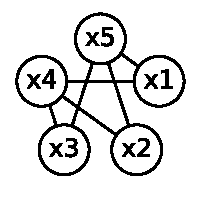
\includegraphics[width=40mm]{img/f372738d3845db182fe0b4a3eced9bc2ac778c82a1804f5788cce6bb74ea1beb.pdf}
}{}

\slide{Matriks Ketetanggaan}{
	\[
		M = \left[ \begin{array}{ccccc}
			0 & 0 & 0 & 1 & 1 \\
			0 & 0 & 0 & 1 & 1 \\
			0 & 0 & 0 & 1 & 1 \\
			1 & 1 & 1 & 0 & 0 \\
			1 & 1 & 1 & 0 & 0
		\end{array} \right]
	\]
}{}

\slide{Matriks Jarak}{
	\[
		D^{(V)} = \left[ \begin{array}{ccccc}
			0 & 2 & 2 & 1 & 1 \\
			2 & 0 & 2 & 1 & 1 \\
			2 & 2 & 0 & 1 & 1 \\
			1 & 1 & 1 & 0 & 2 \\
			1 & 1 & 1 & 2 & 0
		\end{array} \right]
	\]
}{}

\slide{Representasi}{
	\[
		D^{(V)} = \left[ \begin{array}{ccccc}
			r(x_1|V) & r(x_2|V) & r(x_3|V) & r(x_4|V) & r(x_5|V)
		\end{array} \right]
	\]
}{}

\slide{Representasi}{
	\justifying
	\[
		\left[ \begin{array}{ccccc}
			\rowcolor{yellow} 0 & 2 & 2 & 1 & 1 \\
			2 & 0 & 2 & 1 & 1 \\
			2 & 2 & 0 & 1 & 1 \\
			\rowcolor{yellow} 1 & 1 & 1 & 0 & 2 \\
			\rowcolor{yellow} 1 & 1 & 1 & 2 & 0
		\end{array} \right]
	\]
	\vspace{1em} \\
	\(W = \{x_1, x_4, x_5\}\)
	\[
		\left[ \begin{array}{ccccc}
			r(x_1|W) & r(x_2|W) & r(x_3|W) & r(x_4|W) & r(x_5|W)
		\end{array} \right]
	\]
}{}

\slide{\foreign{Distance Similarity Matrix}}{
	\let\oldTrue\True
	\renewcommand{\True}{\cellcolor{pink}\oldTrue}
	\resizebox{\textwidth}{!}{
	\(
		B^{(V)} = \left[ \begin{array}{c@{\enspace}c@{\enspace}c@{\enspace}c@{\enspace}c@{\enspace}c@{\enspace}c@{\enspace}c@{\enspace}c@{\enspace}c@{\enspace}}
			\False & \False & \False & \False &  \True & \False & \False & \False & \False &  \True \\
			\False &  \True & \False & \False & \False & \False & \False & \False & \False &  \True \\
			 \True & \False & \False & \False & \False & \False & \False & \False & \False &  \True \\
			 \True &  \True & \False & \False &  \True & \False & \False & \False & \False & \False \\
			 \True &  \True & \False & \False &  \True & \False & \False & \False & \False & \False
		\end{array} \right]
	\)
	}
}{}

\slide{\foreign{Invalid Resolving Set}}{
	\justifying
	\let\oldTrue\True
	\renewcommand{\True}{\cellcolor{pink}\oldTrue}
	\(W = \{x_1, x_4, x_5\}\)
	\vspace{1em} \\
	\resizebox{\textwidth}{!}{
	\(
		\left[ \begin{array}{c@{\enspace}c@{\enspace}c@{\enspace}c@{\enspace}c@{\enspace}c@{\enspace}c@{\enspace}c@{\enspace}c@{\enspace}c@{\enspace}}
			\False & \False & \False & \False &  \True & \False & \False & \False & \False &  \True \\
			 \True &  \True & \False & \False &  \True & \False & \False & \False & \False & \False \\
			 \True &  \True & \False & \False &  \True & \False & \False & \False & \False & \False
		\end{array} \right]
	\)
	}
}{}

\slide{\foreign{Resolving Set}}{
	\justifying
	\let\oldTrue\True
	\renewcommand{\True}{\cellcolor{pink}\oldTrue}
	\(W = \{x_1, x_4, x_5\}\)
	\vspace{1em} \\
	\resizebox{\textwidth}{!}{
	\(
		B^{(V)} = \left[ \begin{array}{c@{\enspace}c@{\enspace}c@{\enspace}c@{\enspace}c@{\enspace}c@{\enspace}c@{\enspace}c@{\enspace}c@{\enspace}c@{\enspace}}
			\False & \False & \False & \False &  \True & \False & \False & \False & \False &  \True \\
			 \True & \False & \False & \False & \False & \False & \False & \False & \False &  \True \\
			 \True &  \True & \False & \False &  \True & \False & \False & \False & \False & \False
		\end{array} \right]
	\)
	}
}{}

\slide{\foreign{Subset of Invalid Resolving Set}}{
	\justifying
	\let\oldTrue\True
	\renewcommand{\True}{\cellcolor{pink}\oldTrue}
	\(W = \{x_1, x_4, x_5\}\)
	\vspace{1em} \\
	\resizebox{\textwidth}{!}{
	\(
		\left[ \begin{array}{c@{\enspace}c@{\enspace}c@{\enspace}c@{\enspace}c@{\enspace}c@{\enspace}c@{\enspace}c@{\enspace}c@{\enspace}c@{\enspace}}
			\False & \False & \False & \False &  \True & \False & \False & \False & \False &  \True \\
			 \True &  \True & \False & \False &  \True & \False & \False & \False & \False & \False \\
			 \True &  \True & \False & \False &  \True & \False & \False & \False & \False & \False
		\end{array} \right]
	\)
	}
	\vspace{2em} \\
	\(W = \{x_1, x_4\}\)
	\vspace{1em} \\
	\resizebox{\textwidth}{!}{
	\(
		\left[ \begin{array}{c@{\enspace}c@{\enspace}c@{\enspace}c@{\enspace}c@{\enspace}c@{\enspace}c@{\enspace}c@{\enspace}c@{\enspace}c@{\enspace}}
			\False & \False & \False & \False &  \True & \False & \False & \False & \False &  \True \\
			 \True &  \True & \False & \False &  \True & \False & \False & \False & \False & \False
		\end{array} \right]
	\)
	}
}{}

\slide{\foreign{Reduced Distance Similarity Matrix}}{
	\[
		P^{(V)} = \left[ \begin{array}{ccccc}
			\False & \False &  \True &  \True \\
			\False &  \True & \False &  \True \\
			 \True & \False & \False &  \True \\
			 \True &  \True &  \True & \False \\
			 \True &  \True &  \True & \False \\
		\end{array} \right]
	\]
}{}

\outline{3}

\slide{\foreign{Constraint Brute-force}}{
	\justifying

	\[
		\left[ \begin{array}{ccccc}
			\False & \False &  \True &  \True \\
			\False &  \True & \False &  \True \\
			 \True & \False & \False &  \True \\
			 \True &  \True &  \True & \False \\
			 \True &  \True &  \True & \False \\
		\end{array} \right]
		\enspace \to \enspace
		\begin{array}{c}
			\{x_3, x_4, x_5\} \\
			\{x_2, x_4, x_5\} \\
			\{x_1, x_4, x_5\} \\
			\{x_1, x_2, x_3\}
		\end{array}
	\]

	Untuk menentukan apakah sembarang \(W \subseteq V\) merupakan sebuah \foreign{resolving set}, cukup uji habis bahwa \(W\) bukanlah himpunan bagian tak sejati dari seluruh kolom \foreign{reduced distance similarity matrix}.
}{}

\slide{Algoritma \foreign{Brute-force}}{
	\begin{enumerate}
		\item Mulai variabel \(k\) dari banyaknya simpul, yaitu \(k := |V|\).

		\item Selama \(k \geq 0\):
		\begin{enumerate}
			\item Cari satu saja himpunan \(W \subseteq V\) berkardinalitas \(k\) yang merupakan \foreign{resolving set}, kemudian lompat ke tahap (2c).

			\item Bila tidak ditemukan, lompat ke tahap (3).

			\item Kurangi \(k\) sebanyak satu, yaitu \(k := k - 1\).
		\end{enumerate}

		\item Simpulkan bahwa \(k + 1\) adalah dimensi metrik.
	\end{enumerate}
}{}

\slide{\foreign{Constraint Boolean Satisfiability}}{
	\begin{minipage}[t]{.14\textwidth}
	\[
		\begin{array}{c}
			\False \\
			\False \\
			 \True \\
			 \True \\
			 \True
		\end{array}
	\]
	\end{minipage}
	\hfill
	\begin{minipage}[t]{.84\textwidth}
		\vspace{0pt}
		\setlength{\parskip}{.3\baselineskip}

		\foreign{Invalid resolving set} untuk kolom di kiri adalah \(\{x_3, x_4, x_5\}\).

		Bentuk \foreign{constraint} yang persis satu-satu dengan himpunan tersebut adalah \(\neg x_1 \wedge \neg x_2 \wedge x_3 \wedge x_4 \wedge x_5\).

		Bentuk \foreign{constraint} yang ruang solusinya adalah himpunan tersebut dan seluruh himpunan bagiannya adalah \(\neg x_1 \wedge \neg x_2\).

		Dengan demikian, sebuah \foreign{resolving set} haruslah memenuhi kebalikan dari \foreign{constraint} tersebut, yaitu \(x_1 \vee x_2\).
	\end{minipage}
}{}

\slide{\foreign{Constraint Boolean Satisfiability}}{
	\[
		\begin{array}{c}
			x_1 \vee x_2 \\
			x_1 \vee x_3 \\
			x_2 \vee x_3 \\
			x_4 \vee x_5
		\end{array}
	\]
}{}

\slide{\foreign{Constraint Boolean Satisfiability}}{
	\[
		\begin{array}{c}
			x_1 \vee x_2 \vee x_3 \vee x_4 \vee x_5 \\ [4pt]
			x_3 \vee x_4 \vee x_5 \implies x_1 \vee x_2 \\
			x_2 \vee x_4 \vee x_5 \implies x_1 \vee x_3 \\
			x_1 \vee x_4 \vee x_5 \implies x_2 \vee x_3 \\
			x_1 \vee x_2 \vee x_3 \implies x_4 \vee x_5
		\end{array}
	\]
}{}

\slide{\foreign{Constraint Linear Integer Arithmetic}}{
	\[
		\begin{array}{c}
			x_1 + x_2 \geq 1 \\
			x_1 + x_3 \geq 1 \\
			x_2 + x_3 \geq 1 \\
			x_4 + x_5 \geq 1 \\ [4pt]
			0 \leq x_1 \leq 1,\enspace
			0 \leq x_2 \leq 1,\enspace
			0 \leq x_3 \leq 1,\enspace
			0 \leq x_4 \leq 1,\enspace
			0 \leq x_5 \leq 1
		\end{array}
	\]
}{}

\slide{\foreign{Constraint Linear Integer Arithmetic}}{
	\[
		\begin{array}{c}
			x_1 + x_2 + x_3 + x_4 + x_5 = k \\ [4pt]
			x_3 + x_4 + x_5 \leq k - 1 \\
			x_2 + x_4 + x_5 \leq k - 1 \\
			x_1 + x_4 + x_5 \leq k - 1 \\
			x_1 + x_2 + x_3 \leq k - 1 \\ [4pt]
			0 \leq x_1 \leq 1,\enspace
			0 \leq x_2 \leq 1,\enspace
			0 \leq x_3 \leq 1,\enspace
			0 \leq x_4 \leq 1,\enspace
			0 \leq x_5 \leq 1
		\end{array}
	\]
}{}

\slide{\foreign{Constraint Pseudo Boolean}}{
	\[
		\begin{array}{c}
			x_1 + x_2 + x_3 + x_4 + x_5 = k \\ [4pt]
			x_3 + x_4 + x_5 \leq k - 1 \\
			x_2 + x_4 + x_5 \leq k - 1 \\
			x_1 + x_4 + x_5 \leq k - 1 \\
			x_1 + x_2 + x_3 \leq k - 1
		\end{array}
	\]
}{}

\slide{Algoritma \foreign{Satisfiability Modulo Theories}}{
	\begin{enumerate}
		\item Mulai variabel \(k\) dari banyaknya simpul, yaitu \(k := |V|\).

		\item Selama \(k \geq 0\):
		\begin{enumerate}
			\item Cari \foreign{model} berkardinalitas \(k\) yang memenuhi \foreign{constraint}, kemudian lompat ke tahap (2c).

			\item Bila didapatkan \foreign{unsatisfiable}, lompat ke tahap (3).

			\item Kurangi \(k\) sebanyak satu, yaitu \(k := k - 1\).
		\end{enumerate}

		\item Simpulkan bahwa \(k + 1\) adalah dimensi metrik.
	\end{enumerate}
}{}

\outline{4}

\slide{Implementasi}{
}{}

\slide{Batasan Eksekusi}{
}{}

\slide{Data}{
	\resizebox{.275\linewidth}{!}{
		\begin{tabular}{|c|c|}
			\hline
			Graf Bersimpul & Banyak Graf \\ \hline
			2              & 1           \\ \hline
			3              & 2           \\ \hline
			4              & 6           \\ \hline
			5              & 21          \\ \hline
			6              & 112         \\ \hline
			7              & 853         \\ \hline
			8              & 11117       \\ \hline
			9              & 261080      \\ \hline
			10             & 50          \\ \hline
			15             & 50          \\ \hline
			20             & 50          \\ \hline
			25             & 50          \\ \hline
			30             & 50          \\ \hline
			35             & 50          \\ \hline
			40             & 50          \\ \hline
			45             & 50          \\ \hline
			50             & 50          \\ \hline
		\end{tabular}
	}
}{}

\outline{5}

\slide{Frekuensi untuk Graf Kecil}{
	\begin{tabular}{|c|rrrrrrrr|}
		\hline \multirow{2}{*}{\begin{tabular}[c]{@{}c@{}}Dimensi\\ Metrik\end{tabular}} & \multicolumn{8}{c|}{Graf Bersimpul} \\ \cline{2-9} & \multicolumn{1}{c|}{2} & \multicolumn{1}{c|}{3} & \multicolumn{1}{c|}{4} & \multicolumn{1}{c|}{5} & \multicolumn{1}{c|}{6} & \multicolumn{1}{c|}{7} & \multicolumn{1}{c|}{8} & \multicolumn{1}{c|}{9} \\ \hline 1 & \multicolumn{1}{r|}{1} & \multicolumn{1}{r|}{1} & \multicolumn{1}{r|}{1} & \multicolumn{1}{r|}{1} & \multicolumn{1}{r|}{1} & \multicolumn{1}{r|}{1} & \multicolumn{1}{r|}{1} & 1 \\ \hline 2 & \multicolumn{1}{r|}{} & \multicolumn{1}{r|}{1} & \multicolumn{1}{r|}{4} & \multicolumn{1}{r|}{13} & \multicolumn{1}{r|}{62} & \multicolumn{1}{r|}{275} & \multicolumn{1}{r|}{1710} & 12061 \\ \hline 3 & \multicolumn{1}{r|}{} & \multicolumn{1}{r|}{} & \multicolumn{1}{r|}{1} & \multicolumn{1}{r|}{6} & \multicolumn{1}{r|}{39} & \multicolumn{1}{r|}{488} & \multicolumn{1}{r|}{8116} & 216432 \\ \hline 4 & \multicolumn{1}{r|}{} & \multicolumn{1}{r|}{} & \multicolumn{1}{r|}{} & \multicolumn{1}{r|}{1} & \multicolumn{1}{r|}{9} & \multicolumn{1}{r|}{77} & \multicolumn{1}{r|}{1145} & 29958 \\ \hline 5 & \multicolumn{1}{r|}{} & \multicolumn{1}{r|}{} & \multicolumn{1}{r|}{} & \multicolumn{1}{r|}{} & \multicolumn{1}{r|}{1} & \multicolumn{1}{r|}{11} & \multicolumn{1}{r|}{130} & 2415 \\ \hline 6 & \multicolumn{1}{r|}{} & \multicolumn{1}{r|}{} & \multicolumn{1}{r|}{} & \multicolumn{1}{r|}{} & \multicolumn{1}{r|}{} & \multicolumn{1}{r|}{1} & \multicolumn{1}{r|}{14} & 196 \\ \hline 7 & \multicolumn{1}{r|}{} & \multicolumn{1}{r|}{} & \multicolumn{1}{r|}{} & \multicolumn{1}{r|}{} & \multicolumn{1}{r|}{} & \multicolumn{1}{r|}{} & \multicolumn{1}{r|}{1} & 16 \\ \hline 8 & \multicolumn{1}{r|}{} & \multicolumn{1}{r|}{} & \multicolumn{1}{r|}{} & \multicolumn{1}{r|}{} & \multicolumn{1}{r|}{} & \multicolumn{1}{r|}{} & \multicolumn{1}{r|}{} & 1 \\ \hline
	\end{tabular}
}{}

\slide{Frekuensi untuk Graf Kecil}{
	\begin{tabular}{|c|rrrrrrrr|}
		\hline \multirow{2}{*}{\begin{tabular}[c]{@{}c@{}}Dimensi\\ Metrik Sisi\end{tabular}} & \multicolumn{8}{c|}{Graf Bersimpul} \\ \cline{2-9} & \multicolumn{1}{c|}{2} & \multicolumn{1}{c|}{3} & \multicolumn{1}{c|}{4} & \multicolumn{1}{c|}{5} & \multicolumn{1}{c|}{6} & \multicolumn{1}{c|}{7} & \multicolumn{1}{c|}{8} & \multicolumn{1}{c|}{9} \\ \hline 0 & \multicolumn{1}{r|}{1} & \multicolumn{1}{r|}{} & \multicolumn{1}{r|}{} & \multicolumn{1}{r|}{} & \multicolumn{1}{r|}{} & \multicolumn{1}{r|}{} & \multicolumn{1}{r|}{} & \\ \hline 1 & \multicolumn{1}{r|}{} & \multicolumn{1}{r|}{1} & \multicolumn{1}{r|}{1} & \multicolumn{1}{r|}{1} & \multicolumn{1}{r|}{1} & \multicolumn{1}{r|}{1} & \multicolumn{1}{r|}{1} & 1 \\ \hline 2 & \multicolumn{1}{r|}{} & \multicolumn{1}{r|}{1} & \multicolumn{1}{r|}{3} & \multicolumn{1}{r|}{6} & \multicolumn{1}{r|}{17} & \multicolumn{1}{r|}{40} & \multicolumn{1}{r|}{108} & 292 \\ \hline 3 & \multicolumn{1}{r|}{} & \multicolumn{1}{r|}{} & \multicolumn{1}{r|}{2} & \multicolumn{1}{r|}{9} & \multicolumn{1}{r|}{38} & \multicolumn{1}{r|}{198} & \multicolumn{1}{r|}{1148} & 7414 \\ \hline 4 & \multicolumn{1}{r|}{} & \multicolumn{1}{r|}{} & \multicolumn{1}{r|}{} & \multicolumn{1}{r|}{5} & \multicolumn{1}{r|}{42} & \multicolumn{1}{r|}{330} & \multicolumn{1}{r|}{3566} & 49742 \\ \hline 5 & \multicolumn{1}{r|}{} & \multicolumn{1}{r|}{} & \multicolumn{1}{r|}{} & \multicolumn{1}{r|}{} & \multicolumn{1}{r|}{14} & \multicolumn{1}{r|}{236} & \multicolumn{1}{r|}{4081} & 97009 \\ \hline 6 & \multicolumn{1}{r|}{} & \multicolumn{1}{r|}{} & \multicolumn{1}{r|}{} & \multicolumn{1}{r|}{} & \multicolumn{1}{r|}{} & \multicolumn{1}{r|}{48} & \multicolumn{1}{r|}{1995} & 78723 \\ \hline 7 & \multicolumn{1}{r|}{} & \multicolumn{1}{r|}{} & \multicolumn{1}{r|}{} & \multicolumn{1}{r|}{} & \multicolumn{1}{r|}{} & \multicolumn{1}{r|}{} & \multicolumn{1}{r|}{218} & 26401 \\ \hline 8 & \multicolumn{1}{r|}{} & \multicolumn{1}{r|}{} & \multicolumn{1}{r|}{} & \multicolumn{1}{r|}{} & \multicolumn{1}{r|}{} & \multicolumn{1}{r|}{} & \multicolumn{1}{r|}{} & 1498 \\ \hline
	\end{tabular}
}{}

\slide{Gambaran Distribusi}{
	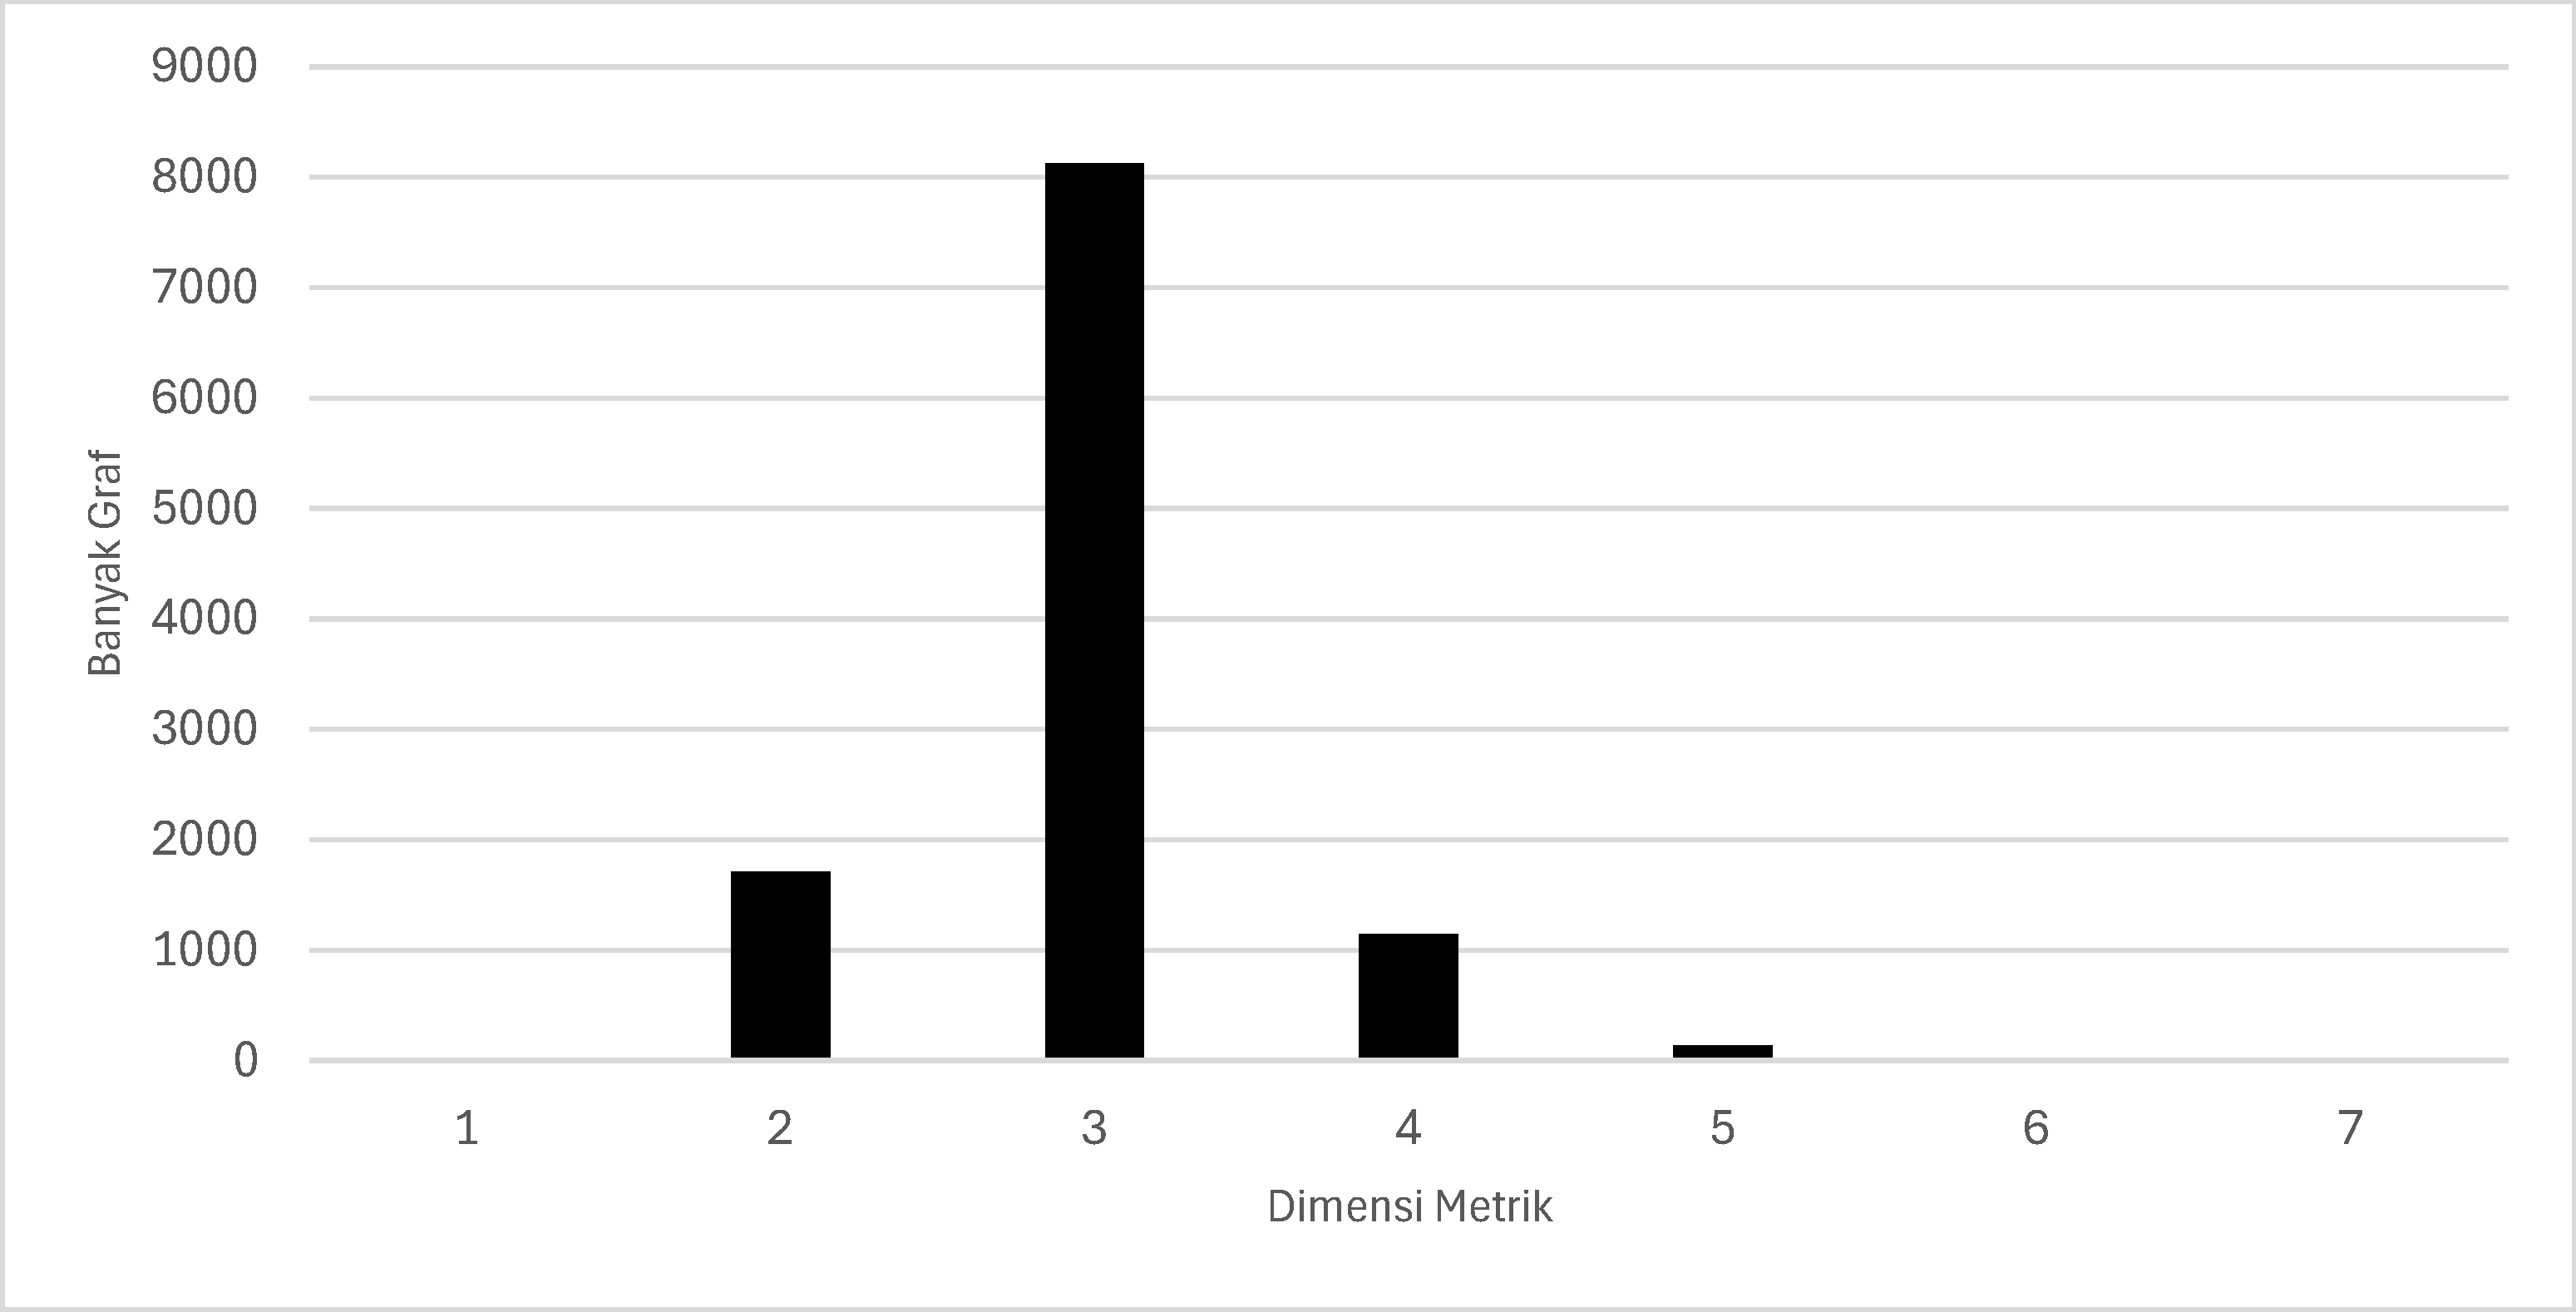
\includegraphics[width=.8\linewidth]{img/hist-md-8.pdf}

	Histogram Dimensi Metrik Graf Bersimpul 8
}{}

\slide{Gambaran Distribusi}{
	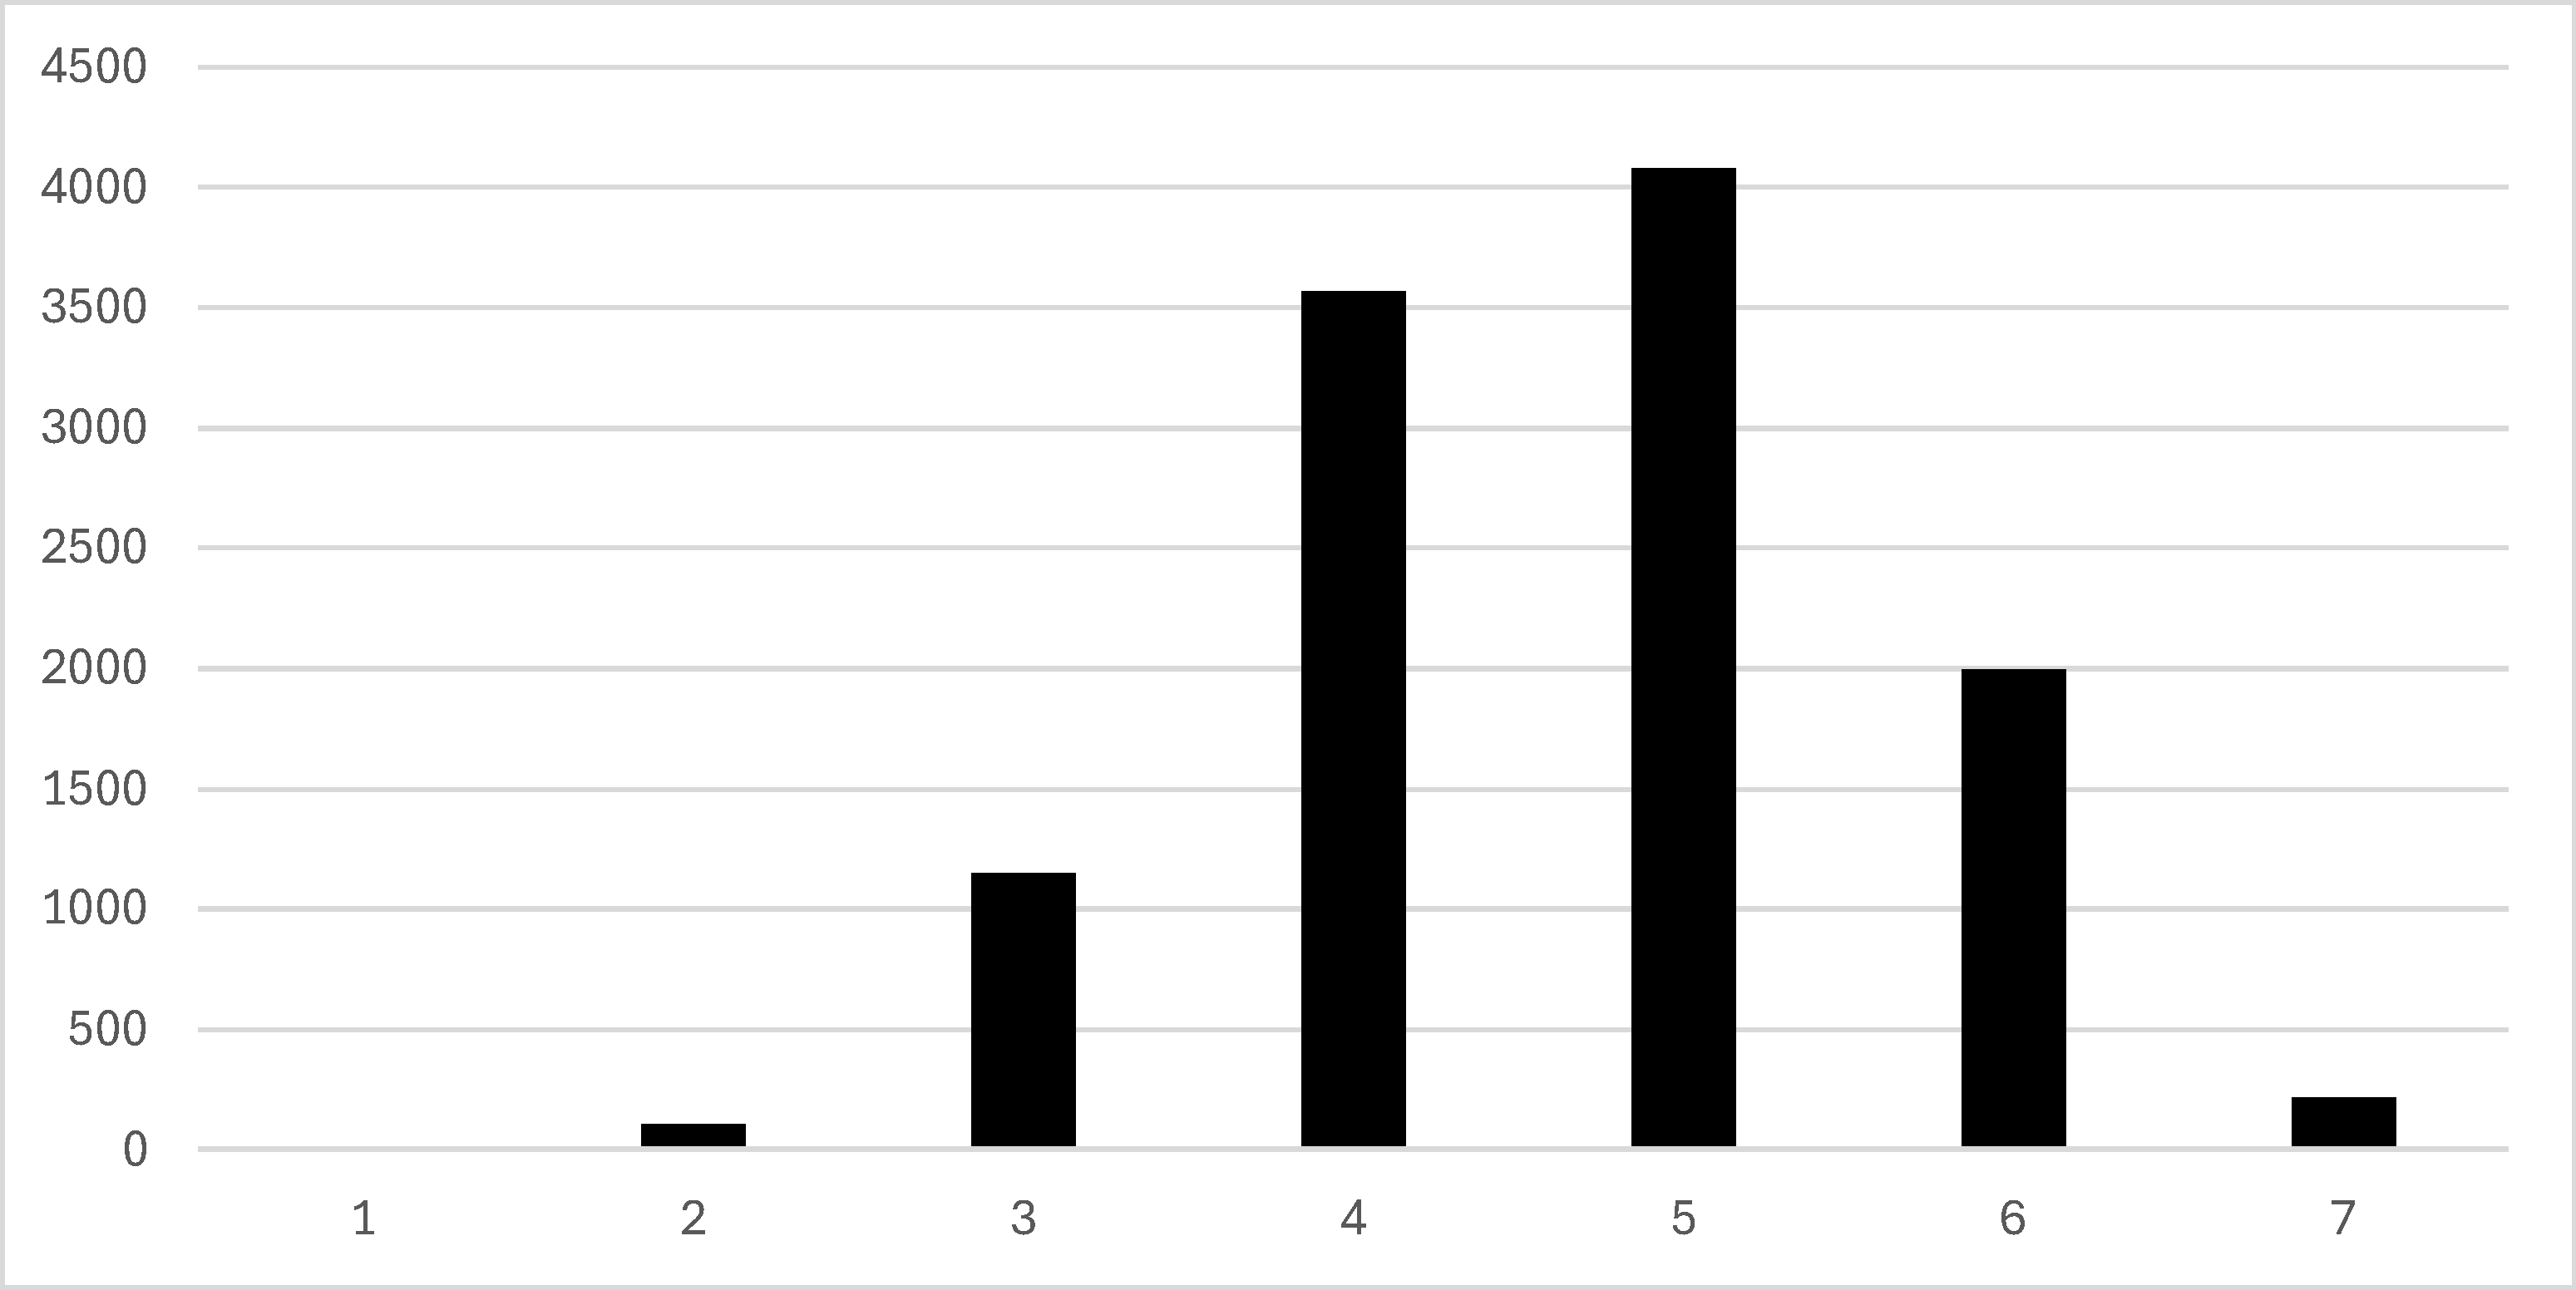
\includegraphics[width=.8\linewidth]{img/hist-emd-8.pdf}

	Histogram Dimensi Metrik Sisi Graf Bersimpul 8
}{}

\slide{Rata-rata Waktu untuk Graf Kecil}{
	\resizebox{\linewidth}{!}{
		\begin{tabular}{|c|c|r|r|r|r|}
			\hline \begin{tabular}[c]{@{}c@{}}Dimensi\\ Metrik\end{tabular} & \begin{tabular}[c]{@{}c@{}}Graf\\ Bersimpul\end{tabular} & \multicolumn{1}{c|}{\foreign{Brute-force}} & \multicolumn{1}{c|}{\begin{tabular}[c]{@{}c@{}}\foreign{Boolean}\\ \foreign{Satisfiability}\end{tabular}} & \multicolumn{1}{c|}{\begin{tabular}[c]{@{}c@{}}\foreign{Linear Integer}\\ \foreign{Arithmetic}\end{tabular}} & \multicolumn{1}{c|}{\begin{tabular}[c]{@{}c@{}}\foreign{Pseudo}\\ \foreign{Boolean}\end{tabular}} \\ \hline 1 & 2 & .156965 & .174657 & .186278 & .170794 \\ \hline 1 & 3 & .153144 & .173771 & .061201 & .003076 \\ \hline 2 & 4 & .000947 & .009032 & .028977 & .003894 \\ \hline 2 & 5 & .001206 & .006250 & .034587 & .005617 \\ \hline 2 & 6 & .001573 & .008373 & .043509 & .007274 \\ \hline 3 & 7 & .002507 & .011181 & .052244 & .010301 \\ \hline 3 & 8 & .002948 & .014158 & .068935 & .014817 \\ \hline 3 & 9 & .003770 & .018461 & .093387 & .021154 \\ \hline
		\end{tabular}
	}
}{}

\slide{Rata-rata Waktu untuk Graf Kecil}{
	\resizebox{\linewidth}{!}{
		\begin{tabular}{|c|c|r|r|r|r|}
			\hline \begin{tabular}[c]{@{}c@{}}Dimensi\\ Metrik Sisi\end{tabular} & \begin{tabular}[c]{@{}c@{}}Graf\\ Bersimpul\end{tabular} & \multicolumn{1}{c|}{\foreign{Brute-force}} & \multicolumn{1}{c|}{\begin{tabular}[c]{@{}c@{}}\foreign{Boolean}\\ \foreign{Satisfiability}\end{tabular}} & \multicolumn{1}{c|}{\begin{tabular}[c]{@{}c@{}}\foreign{Linear Integer}\\ \foreign{Arithmetic}\end{tabular}} & \multicolumn{1}{c|}{\begin{tabular}[c]{@{}c@{}}\foreign{Pseudo}\\ \foreign{Boolean}\end{tabular}} \\ \hline 0 & 2 & .000783 & .003237 & .009080 & .002883 \\ \hline 1 & 3 & .000899 & .004708 & .020789 & .003183 \\ \hline 2 & 4 & .000792 & .005288 & .024364 & .003950 \\ \hline 3 & 5 & .001399 & .007340 & .029201 & .006055 \\ \hline 4 & 6 & .002330 & .009507 & .033777 & .009077 \\ \hline 4 & 7 & .003574 & .012815 & .048816 & .013481 \\ \hline 5 & 8 & .006108 & .017646 & .059845 & .021366 \\ \hline 5 & 9 & .009322 & .023267 & .087683 & .031534 \\ \hline
		\end{tabular}
	}
}{}

\slide{Tren Waktu untuk Graf Kecil}{
	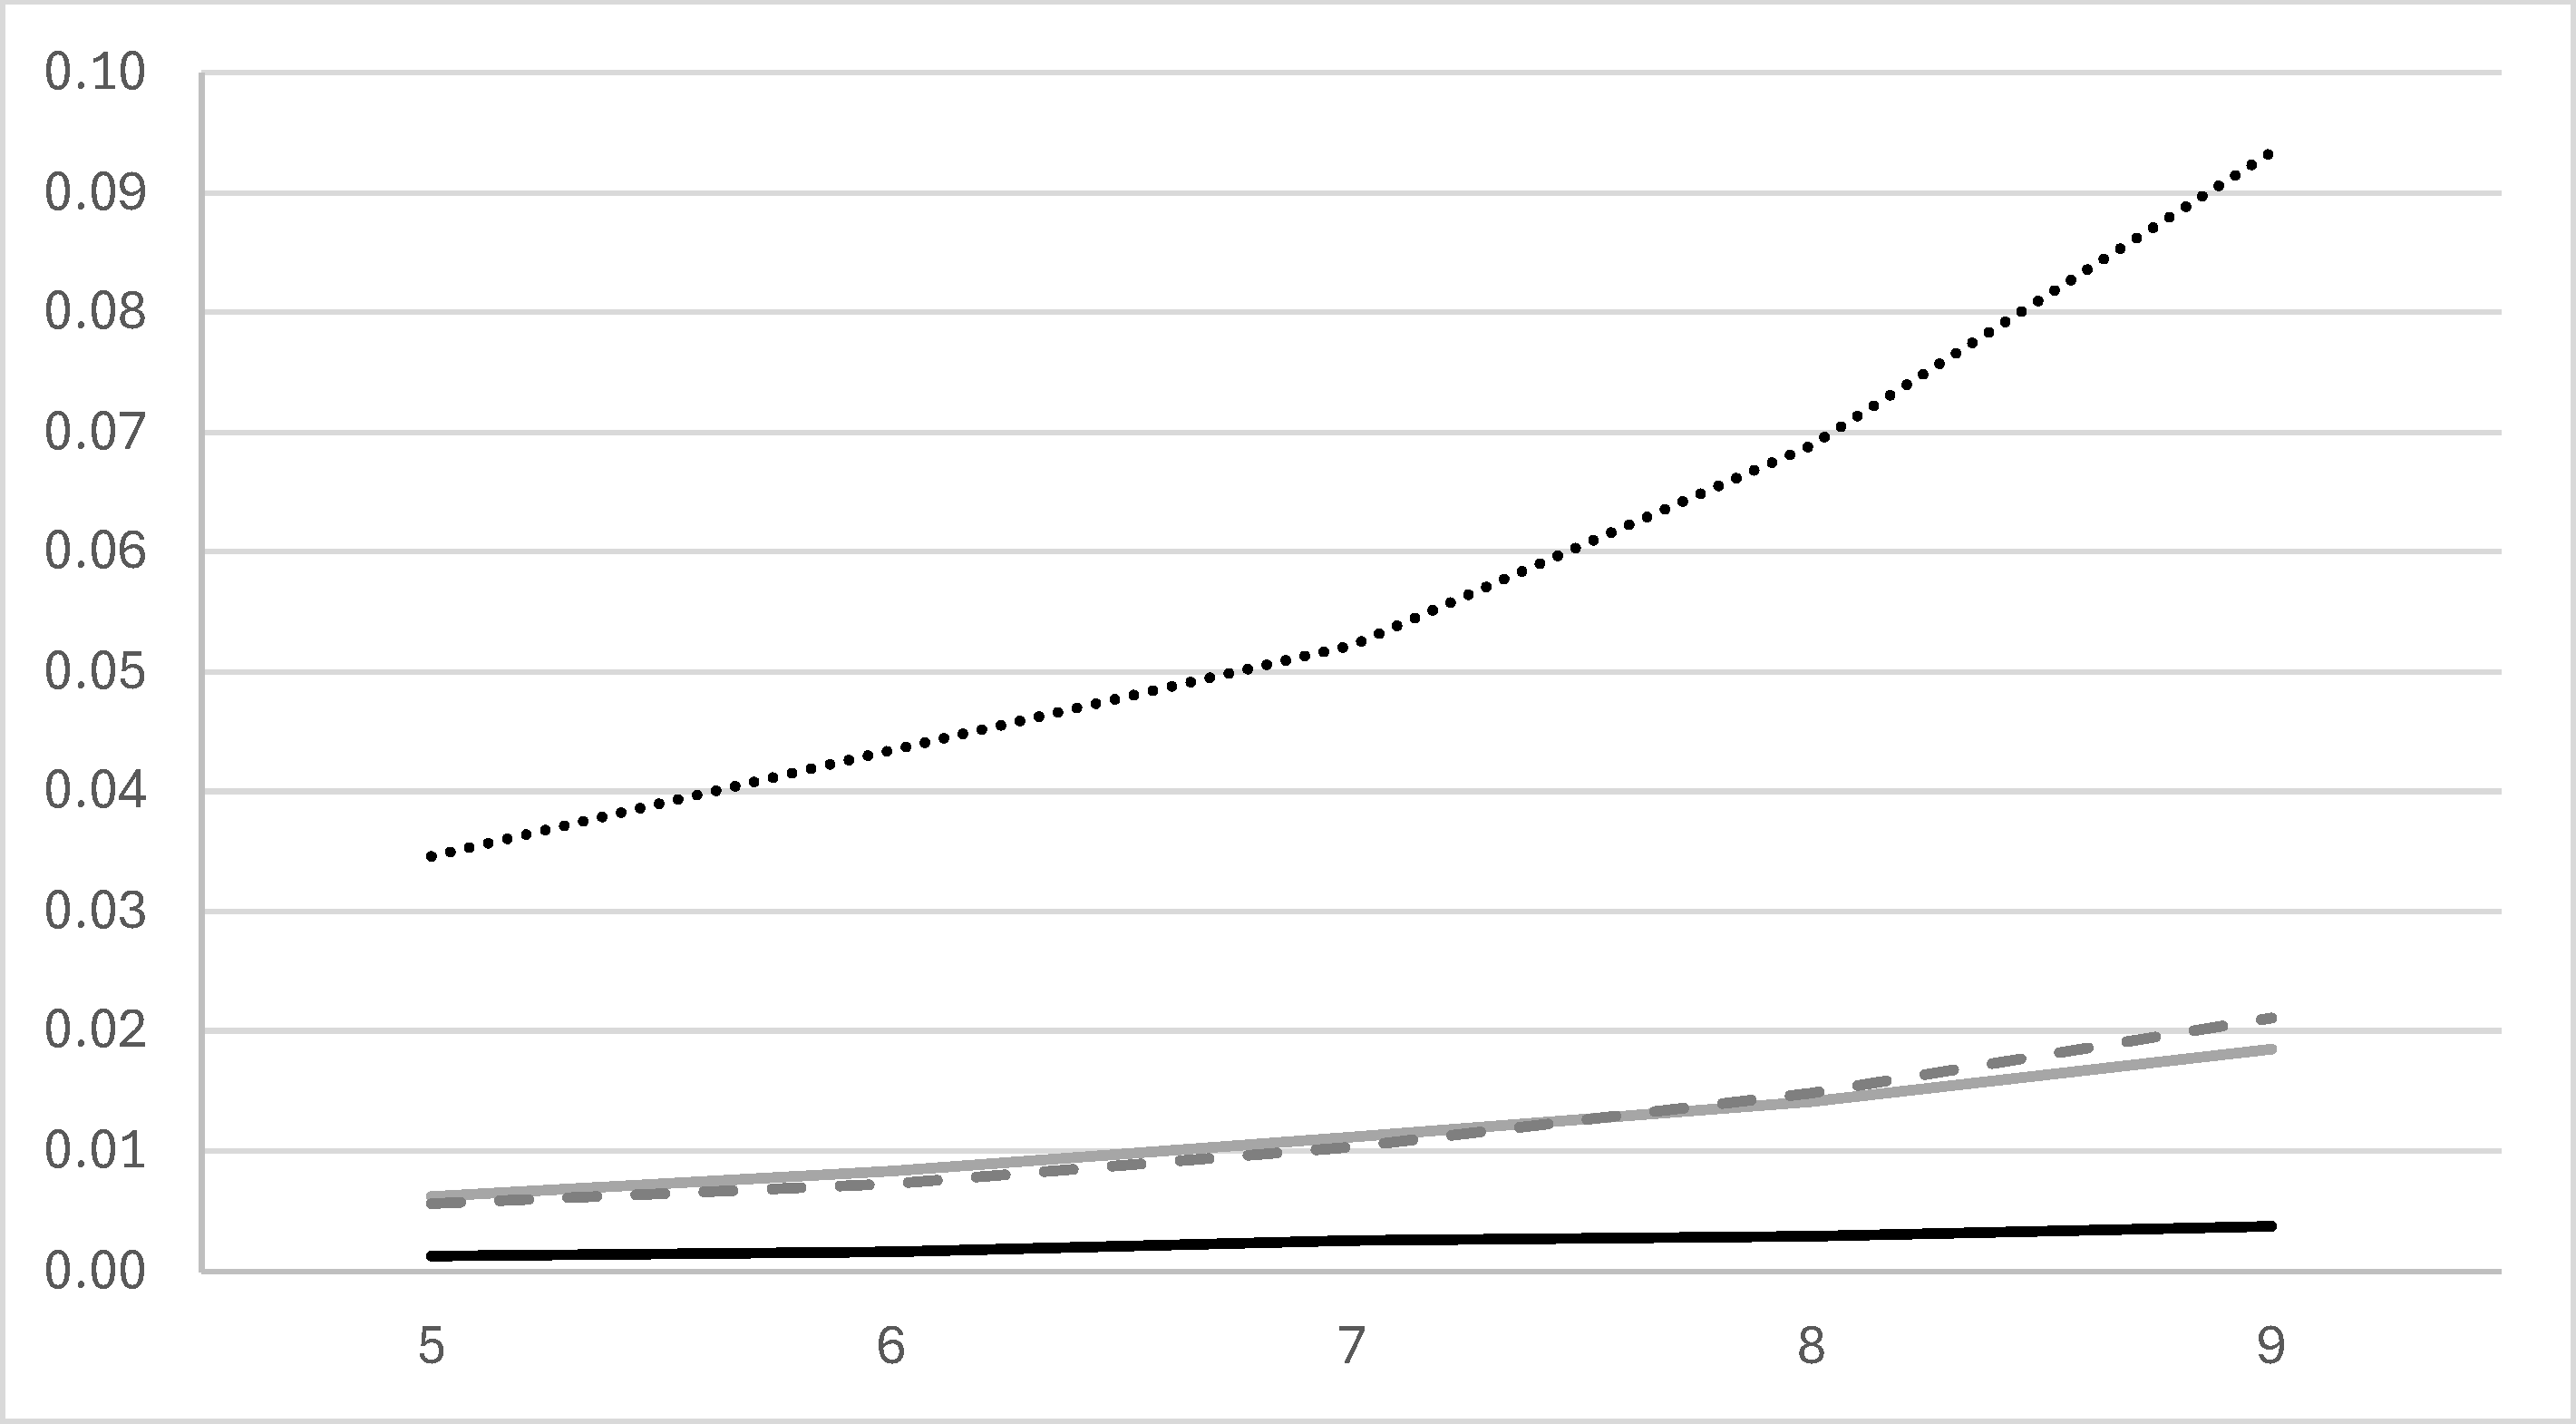
\includegraphics[width=.8\linewidth]{img/trend-md-small.pdf}

	Tren Waktu Eksekusi Dimensi Metrik Graf Kecil
}{}

\slide{Tren Waktu untuk Graf Kecil}{
	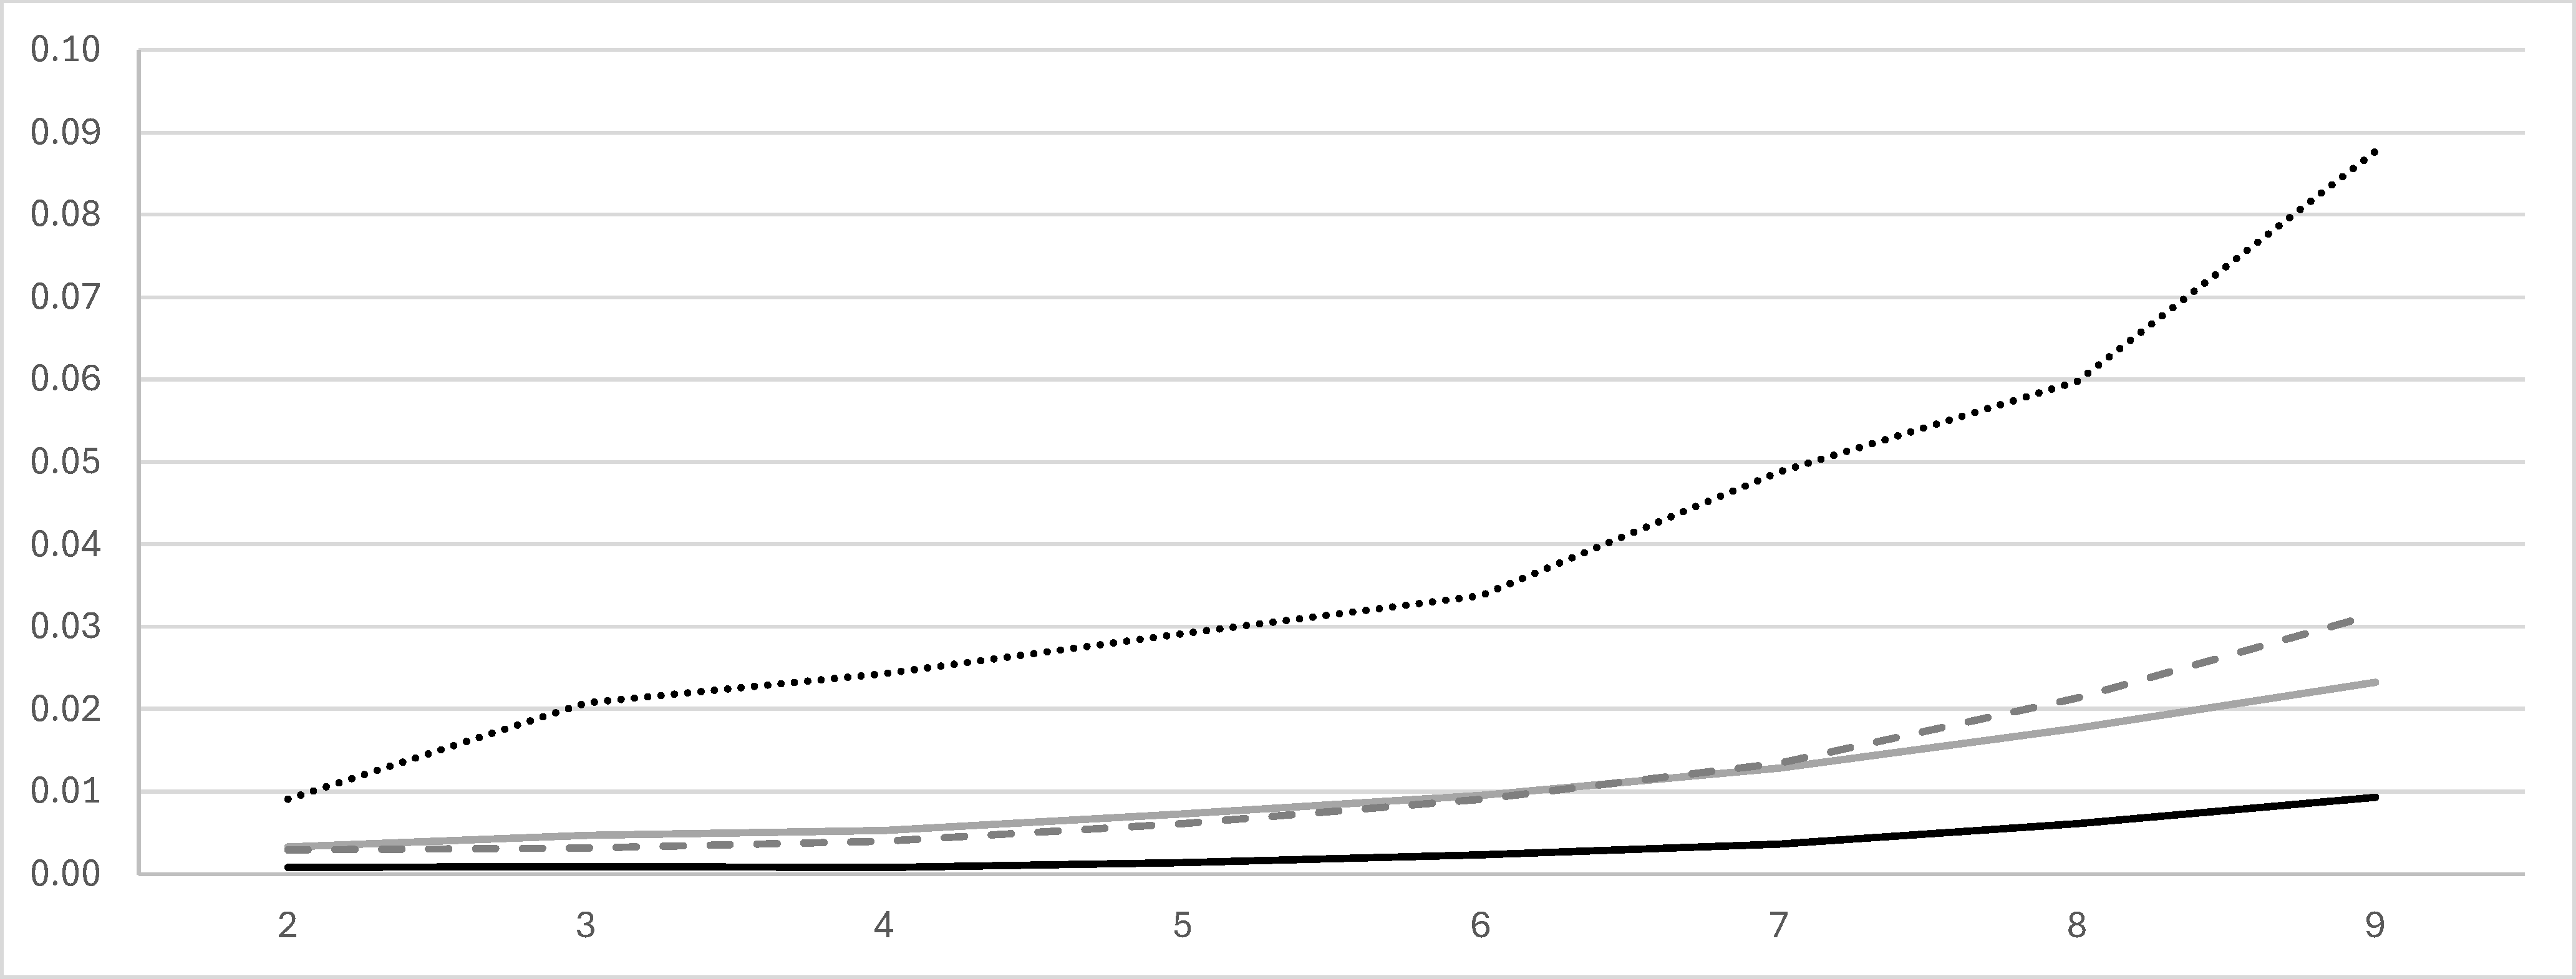
\includegraphics[width=\linewidth]{img/trend-emd-small.pdf}

	Tren Waktu Eksekusi Dimensi Sisi Metrik Graf Kecil
}{}

\slide{Frekuensi untuk Graf Besar}{
	\begin{multicols}{2}
	Frekuensi Dimensi Metrik Graf Besar\\ \foreign{Brute-force}

	\resizebox{\linewidth}{!}{
		\begin{tabular}{|c|lllllllll|}
			\hline \multirow{2}{*}{\begin{tabular}[c]{@{}c@{}}Dimensi\\ Metrik\end{tabular}} & \multicolumn{9}{c|}{Graf Bersimpul} \\ \cline{2-10} & \multicolumn{1}{c|}{10} & \multicolumn{1}{c|}{15} & \multicolumn{1}{c|}{20} & \multicolumn{1}{c|}{25} & \multicolumn{1}{c|}{30} & \multicolumn{1}{c|}{35} & \multicolumn{1}{c|}{40} & \multicolumn{1}{c|}{45} & \multicolumn{1}{c|}{50} \\ \hline 2 & \multicolumn{1}{r|}{1} & \multicolumn{1}{r|}{} & \multicolumn{1}{r|}{} & \multicolumn{1}{r|}{} & \multicolumn{1}{r|}{} & \multicolumn{1}{r|}{} & \multicolumn{1}{r|}{} & \multicolumn{1}{r|}{} & \\ \hline 3 & \multicolumn{1}{r|}{34} & \multicolumn{1}{r|}{} & \multicolumn{1}{r|}{} & \multicolumn{1}{r|}{} & \multicolumn{1}{r|}{} & \multicolumn{1}{r|}{} & \multicolumn{1}{r|}{} & \multicolumn{1}{r|}{} & \\ \hline 4 & \multicolumn{1}{r|}{14} & \multicolumn{1}{r|}{50} & \multicolumn{1}{r|}{4} & \multicolumn{1}{r|}{} & \multicolumn{1}{r|}{} & \multicolumn{1}{r|}{} & \multicolumn{1}{r|}{} & \multicolumn{1}{r|}{} & \\ \hline 5 & \multicolumn{1}{r|}{1} & \multicolumn{1}{r|}{} & \multicolumn{1}{r|}{46} & \multicolumn{1}{r|}{50} & \multicolumn{1}{r|}{4} & \multicolumn{1}{r|}{} & \multicolumn{1}{r|}{} & \multicolumn{1}{r|}{} & \\ \hline 6 & \multicolumn{1}{r|}{} & \multicolumn{1}{r|}{} & \multicolumn{1}{r|}{} & \multicolumn{1}{r|}{} & \multicolumn{1}{r|}{46} & \multicolumn{1}{r|}{50} & \multicolumn{1}{r|}{50} & \multicolumn{1}{r|}{17} & \\ \hline 7 & \multicolumn{1}{r|}{} & \multicolumn{1}{r|}{} & \multicolumn{1}{r|}{} & \multicolumn{1}{r|}{} & \multicolumn{1}{r|}{} & \multicolumn{1}{r|}{} & \multicolumn{1}{r|}{} & \multicolumn{1}{r|}{} & \\ \hline Gagal & \multicolumn{1}{r|}{} & \multicolumn{1}{r|}{} & \multicolumn{1}{r|}{} & \multicolumn{1}{r|}{} & \multicolumn{1}{r|}{} & \multicolumn{1}{r|}{} & \multicolumn{1}{r|}{} & \multicolumn{1}{r|}{33} & 50 \\ \hline
		\end{tabular}
	}

	Frekuensi Dimensi Metrik Graf Besar\\ \foreign{Boolean Satisfiability}

	\resizebox{\linewidth}{!}{
		\begin{tabular}{|c|lllllllll|}
			\hline \multirow{2}{*}{\begin{tabular}[c]{@{}c@{}}Dimensi\\ Metrik\end{tabular}} & \multicolumn{9}{c|}{Graf Bersimpul} \\ \cline{2-10} & \multicolumn{1}{c|}{10} & \multicolumn{1}{c|}{15} & \multicolumn{1}{c|}{20} & \multicolumn{1}{c|}{25} & \multicolumn{1}{c|}{30} & \multicolumn{1}{c|}{35} & \multicolumn{1}{c|}{40} & \multicolumn{1}{c|}{45} & \multicolumn{1}{c|}{50} \\ \hline 2 & \multicolumn{1}{r|}{1} & \multicolumn{1}{r|}{} & \multicolumn{1}{r|}{} & \multicolumn{1}{r|}{} & \multicolumn{1}{r|}{} & \multicolumn{1}{r|}{} & \multicolumn{1}{r|}{} & \multicolumn{1}{r|}{} & \\ \hline 3 & \multicolumn{1}{r|}{34} & \multicolumn{1}{r|}{} & \multicolumn{1}{r|}{} & \multicolumn{1}{r|}{} & \multicolumn{1}{r|}{} & \multicolumn{1}{r|}{} & \multicolumn{1}{r|}{} & \multicolumn{1}{r|}{} & \\ \hline 4 & \multicolumn{1}{r|}{14} & \multicolumn{1}{r|}{50} & \multicolumn{1}{r|}{4} & \multicolumn{1}{r|}{} & \multicolumn{1}{r|}{} & \multicolumn{1}{r|}{} & \multicolumn{1}{r|}{} & \multicolumn{1}{r|}{} & \\ \hline 5 & \multicolumn{1}{r|}{1} & \multicolumn{1}{r|}{} & \multicolumn{1}{r|}{46} & \multicolumn{1}{r|}{50} & \multicolumn{1}{r|}{4} & \multicolumn{1}{r|}{} & \multicolumn{1}{r|}{} & \multicolumn{1}{r|}{} & \\ \hline 6 & \multicolumn{1}{r|}{} & \multicolumn{1}{r|}{} & \multicolumn{1}{r|}{} & \multicolumn{1}{r|}{} & \multicolumn{1}{r|}{46} & \multicolumn{1}{r|}{50} & \multicolumn{1}{r|}{50} & \multicolumn{1}{r|}{14} & \\ \hline 7 & \multicolumn{1}{r|}{} & \multicolumn{1}{r|}{} & \multicolumn{1}{r|}{} & \multicolumn{1}{r|}{} & \multicolumn{1}{r|}{} & \multicolumn{1}{r|}{} & \multicolumn{1}{r|}{} & \multicolumn{1}{r|}{} & \\ \hline Gagal & \multicolumn{1}{r|}{} & \multicolumn{1}{r|}{} & \multicolumn{1}{r|}{} & \multicolumn{1}{r|}{} & \multicolumn{1}{r|}{} & \multicolumn{1}{r|}{} & \multicolumn{1}{r|}{} & \multicolumn{1}{r|}{36} & 50 \\ \hline
		\end{tabular}
	}
	\end{multicols}
}{}

\slide{Frekuensi untuk Graf Besar}{
	\begin{multicols}{2}
	Frekuensi Dimensi Metrik Graf Besar\\ \foreign{Linear Integer Arithmetic}

	\resizebox{\linewidth}{!}{
		\begin{tabular}{|c|lllllllll|}
			\hline \multirow{2}{*}{\begin{tabular}[c]{@{}c@{}}Dimensi\\ Metrik\end{tabular}} & \multicolumn{9}{c|}{Graf Bersimpul} \\ \cline{2-10} & \multicolumn{1}{c|}{10} & \multicolumn{1}{c|}{15} & \multicolumn{1}{c|}{20} & \multicolumn{1}{c|}{25} & \multicolumn{1}{c|}{30} & \multicolumn{1}{c|}{35} & \multicolumn{1}{c|}{40} & \multicolumn{1}{c|}{45} & \multicolumn{1}{c|}{50} \\ \hline 2 & \multicolumn{1}{r|}{1} & \multicolumn{1}{r|}{} & \multicolumn{1}{r|}{} & \multicolumn{1}{r|}{} & \multicolumn{1}{r|}{} & \multicolumn{1}{r|}{} & \multicolumn{1}{r|}{} & \multicolumn{1}{r|}{} & \\ \hline 3 & \multicolumn{1}{r|}{34} & \multicolumn{1}{r|}{} & \multicolumn{1}{r|}{} & \multicolumn{1}{r|}{} & \multicolumn{1}{r|}{} & \multicolumn{1}{r|}{} & \multicolumn{1}{r|}{} & \multicolumn{1}{r|}{} & \\ \hline 4 & \multicolumn{1}{r|}{14} & \multicolumn{1}{r|}{50} & \multicolumn{1}{r|}{4} & \multicolumn{1}{r|}{} & \multicolumn{1}{r|}{} & \multicolumn{1}{r|}{} & \multicolumn{1}{r|}{} & \multicolumn{1}{r|}{} & \\ \hline 5 & \multicolumn{1}{r|}{1} & \multicolumn{1}{r|}{} & \multicolumn{1}{r|}{46} & \multicolumn{1}{r|}{50} & \multicolumn{1}{r|}{4} & \multicolumn{1}{r|}{} & \multicolumn{1}{r|}{} & \multicolumn{1}{r|}{} & \\ \hline 6 & \multicolumn{1}{r|}{} & \multicolumn{1}{r|}{} & \multicolumn{1}{r|}{} & \multicolumn{1}{r|}{} & \multicolumn{1}{r|}{46} & \multicolumn{1}{r|}{50} & \multicolumn{1}{r|}{50} & \multicolumn{1}{r|}{23} & \\ \hline 7 & \multicolumn{1}{r|}{} & \multicolumn{1}{r|}{} & \multicolumn{1}{r|}{} & \multicolumn{1}{r|}{} & \multicolumn{1}{r|}{} & \multicolumn{1}{r|}{} & \multicolumn{1}{r|}{} & \multicolumn{1}{r|}{} & \\ \hline Gagal & \multicolumn{1}{r|}{} & \multicolumn{1}{r|}{} & \multicolumn{1}{r|}{} & \multicolumn{1}{r|}{} & \multicolumn{1}{r|}{} & \multicolumn{1}{r|}{} & \multicolumn{1}{r|}{} & \multicolumn{1}{r|}{27} & 50 \\ \hline
		\end{tabular}
	}

	Frekuensi Dimensi Metrik Graf Besar\\ \foreign{Pseudo Boolean}

	\resizebox{\linewidth}{!}{
		\begin{tabular}{|c|lllllllll|}
			\hline \multirow{2}{*}{\begin{tabular}[c]{@{}c@{}}Dimensi\\ Metrik\end{tabular}} & \multicolumn{9}{c|}{Graf Bersimpul} \\ \cline{2-10} & \multicolumn{1}{c|}{10} & \multicolumn{1}{c|}{15} & \multicolumn{1}{c|}{20} & \multicolumn{1}{c|}{25} & \multicolumn{1}{c|}{30} & \multicolumn{1}{c|}{35} & \multicolumn{1}{c|}{40} & \multicolumn{1}{c|}{45} & \multicolumn{1}{c|}{50} \\ \hline 2 & \multicolumn{1}{r|}{1} & \multicolumn{1}{r|}{} & \multicolumn{1}{r|}{} & \multicolumn{1}{r|}{} & \multicolumn{1}{r|}{} & \multicolumn{1}{r|}{} & \multicolumn{1}{r|}{} & \multicolumn{1}{r|}{} & \\ \hline 3 & \multicolumn{1}{r|}{34} & \multicolumn{1}{r|}{} & \multicolumn{1}{r|}{} & \multicolumn{1}{r|}{} & \multicolumn{1}{r|}{} & \multicolumn{1}{r|}{} & \multicolumn{1}{r|}{} & \multicolumn{1}{r|}{} & \\ \hline 4 & \multicolumn{1}{r|}{14} & \multicolumn{1}{r|}{50} & \multicolumn{1}{r|}{4} & \multicolumn{1}{r|}{} & \multicolumn{1}{r|}{} & \multicolumn{1}{r|}{} & \multicolumn{1}{r|}{} & \multicolumn{1}{r|}{} & \\ \hline 5 & \multicolumn{1}{r|}{1} & \multicolumn{1}{r|}{} & \multicolumn{1}{r|}{46} & \multicolumn{1}{r|}{50} & \multicolumn{1}{r|}{4} & \multicolumn{1}{r|}{} & \multicolumn{1}{r|}{} & \multicolumn{1}{r|}{} & \\ \hline 6 & \multicolumn{1}{r|}{} & \multicolumn{1}{r|}{} & \multicolumn{1}{r|}{} & \multicolumn{1}{r|}{} & \multicolumn{1}{r|}{46} & \multicolumn{1}{r|}{50} & \multicolumn{1}{r|}{50} & \multicolumn{1}{r|}{39} & 1 \\ \hline 7 & \multicolumn{1}{r|}{} & \multicolumn{1}{r|}{} & \multicolumn{1}{r|}{} & \multicolumn{1}{r|}{} & \multicolumn{1}{r|}{} & \multicolumn{1}{r|}{} & \multicolumn{1}{r|}{} & \multicolumn{1}{r|}{11} & 49 \\ \hline Gagal & \multicolumn{1}{r|}{} & \multicolumn{1}{r|}{} & \multicolumn{1}{r|}{} & \multicolumn{1}{r|}{} & \multicolumn{1}{r|}{} & \multicolumn{1}{r|}{} & \multicolumn{1}{r|}{} & \multicolumn{1}{r|}{} & \\ \hline
		\end{tabular}
	}
	\end{multicols}
}{}

\slide{Frekuensi untuk Graf Besar}{
	\begin{multicols}{2}
	Frekuensi Dimensi Metrik Sisi Graf\\ Besar \foreign{Brute-force}

	\resizebox{.8\linewidth}{!}{
		\begin{tabular}{|c|lllllllll|}
			\hline \multirow{2}{*}{\begin{tabular}[c]{@{}c@{}}Dimensi\\ Metrik Sisi\end{tabular}} & \multicolumn{9}{c|}{Graf Bersimpul} \\ \cline{2-10} & \multicolumn{1}{c|}{10} & \multicolumn{1}{c|}{15} & \multicolumn{1}{c|}{20} & \multicolumn{1}{c|}{25} & \multicolumn{1}{c|}{30} & \multicolumn{1}{c|}{35} & \multicolumn{1}{c|}{40} & \multicolumn{1}{c|}{45} & \multicolumn{1}{c|}{50} \\ \hline 4 & \multicolumn{1}{r|}{6} & \multicolumn{1}{r|}{} & \multicolumn{1}{r|}{} & \multicolumn{1}{r|}{} & \multicolumn{1}{r|}{} & \multicolumn{1}{r|}{} & \multicolumn{1}{r|}{} & \multicolumn{1}{r|}{} & \\ \hline 5 & \multicolumn{1}{r|}{27} & \multicolumn{1}{r|}{} & \multicolumn{1}{r|}{} & \multicolumn{1}{r|}{} & \multicolumn{1}{r|}{} & \multicolumn{1}{r|}{} & \multicolumn{1}{r|}{} & \multicolumn{1}{r|}{} & \\ \hline 6 & \multicolumn{1}{r|}{13} & \multicolumn{1}{r|}{} & \multicolumn{1}{r|}{} & \multicolumn{1}{r|}{} & \multicolumn{1}{r|}{} & \multicolumn{1}{r|}{} & \multicolumn{1}{r|}{} & \multicolumn{1}{r|}{} & \\ \hline 7 & \multicolumn{1}{r|}{4} & \multicolumn{1}{r|}{11} & \multicolumn{1}{r|}{} & \multicolumn{1}{r|}{} & \multicolumn{1}{r|}{} & \multicolumn{1}{r|}{} & \multicolumn{1}{r|}{} & \multicolumn{1}{r|}{} & \\ \hline 8 & \multicolumn{1}{r|}{} & \multicolumn{1}{r|}{19} & \multicolumn{1}{r|}{} & \multicolumn{1}{r|}{} & \multicolumn{1}{r|}{} & \multicolumn{1}{r|}{} & \multicolumn{1}{r|}{} & \multicolumn{1}{r|}{} & \\ \hline 9 & \multicolumn{1}{r|}{} & \multicolumn{1}{r|}{13} & \multicolumn{1}{r|}{10} & \multicolumn{1}{r|}{} & \multicolumn{1}{r|}{} & \multicolumn{1}{r|}{} & \multicolumn{1}{r|}{} & \multicolumn{1}{r|}{} & \\ \hline 10 & \multicolumn{1}{r|}{} & \multicolumn{1}{r|}{6} & \multicolumn{1}{r|}{19} & \multicolumn{1}{r|}{2} & \multicolumn{1}{r|}{} & \multicolumn{1}{r|}{} & \multicolumn{1}{r|}{} & \multicolumn{1}{r|}{} & \\ \hline 11 & \multicolumn{1}{r|}{} & \multicolumn{1}{r|}{1} & \multicolumn{1}{r|}{10} & \multicolumn{1}{r|}{7} & \multicolumn{1}{r|}{} & \multicolumn{1}{r|}{} & \multicolumn{1}{r|}{} & \multicolumn{1}{r|}{} & \\ \hline 12 & \multicolumn{1}{r|}{} & \multicolumn{1}{r|}{} & \multicolumn{1}{r|}{10} & \multicolumn{1}{r|}{25} & \multicolumn{1}{r|}{} & \multicolumn{1}{r|}{} & \multicolumn{1}{r|}{} & \multicolumn{1}{r|}{} & \\ \hline 13 & \multicolumn{1}{r|}{} & \multicolumn{1}{r|}{} & \multicolumn{1}{r|}{} & \multicolumn{1}{r|}{13} & \multicolumn{1}{r|}{} & \multicolumn{1}{r|}{} & \multicolumn{1}{r|}{} & \multicolumn{1}{r|}{} & \\ \hline 14 & \multicolumn{1}{r|}{} & \multicolumn{1}{r|}{} & \multicolumn{1}{r|}{1} & \multicolumn{1}{r|}{1} & \multicolumn{1}{r|}{} & \multicolumn{1}{r|}{} & \multicolumn{1}{r|}{} & \multicolumn{1}{r|}{} & \\ \hline 15 & \multicolumn{1}{r|}{} & \multicolumn{1}{r|}{} & \multicolumn{1}{r|}{} & \multicolumn{1}{r|}{1} & \multicolumn{1}{r|}{} & \multicolumn{1}{r|}{} & \multicolumn{1}{r|}{} & \multicolumn{1}{r|}{} & \\ \hline 16 & \multicolumn{1}{r|}{} & \multicolumn{1}{r|}{} & \multicolumn{1}{r|}{} & \multicolumn{1}{r|}{} & \multicolumn{1}{r|}{} & \multicolumn{1}{r|}{} & \multicolumn{1}{r|}{} & \multicolumn{1}{r|}{} & \\ \hline 17 & \multicolumn{1}{r|}{} & \multicolumn{1}{r|}{} & \multicolumn{1}{r|}{} & \multicolumn{1}{r|}{} & \multicolumn{1}{r|}{} & \multicolumn{1}{r|}{} & \multicolumn{1}{r|}{} & \multicolumn{1}{r|}{} & \\ \hline 18 & \multicolumn{1}{r|}{} & \multicolumn{1}{r|}{} & \multicolumn{1}{r|}{} & \multicolumn{1}{r|}{} & \multicolumn{1}{r|}{} & \multicolumn{1}{r|}{} & \multicolumn{1}{r|}{} & \multicolumn{1}{r|}{} & \\ \hline Gagal & \multicolumn{1}{r|}{} & \multicolumn{1}{r|}{} & \multicolumn{1}{r|}{} & \multicolumn{1}{r|}{1} & \multicolumn{1}{r|}{50} & \multicolumn{1}{r|}{50} & \multicolumn{1}{r|}{50} & \multicolumn{1}{r|}{50} & 50 \\ \hline
		\end{tabular}
	}

	Frekuensi Dimensi Metrik Sisi Graf\\ Besar \foreign{Boolean Satisfiability}

	\resizebox{.8\linewidth}{!}{
		\begin{tabular}{|c|lllllllll|}
			\hline \multirow{2}{*}{\begin{tabular}[c]{@{}c@{}}Dimensi\\ Metrik Sisi\end{tabular}} & \multicolumn{9}{c|}{Graf Bersimpul} \\ \cline{2-10} & \multicolumn{1}{c|}{10} & \multicolumn{1}{c|}{15} & \multicolumn{1}{c|}{20} & \multicolumn{1}{c|}{25} & \multicolumn{1}{c|}{30} & \multicolumn{1}{c|}{35} & \multicolumn{1}{c|}{40} & \multicolumn{1}{c|}{45} & \multicolumn{1}{c|}{50} \\ \hline 4 & \multicolumn{1}{r|}{6} & \multicolumn{1}{r|}{} & \multicolumn{1}{r|}{} & \multicolumn{1}{r|}{} & \multicolumn{1}{r|}{} & \multicolumn{1}{r|}{} & \multicolumn{1}{r|}{} & \multicolumn{1}{r|}{} & \\ \hline 5 & \multicolumn{1}{r|}{27} & \multicolumn{1}{r|}{} & \multicolumn{1}{r|}{} & \multicolumn{1}{r|}{} & \multicolumn{1}{r|}{} & \multicolumn{1}{r|}{} & \multicolumn{1}{r|}{} & \multicolumn{1}{r|}{} & \\ \hline 6 & \multicolumn{1}{r|}{13} & \multicolumn{1}{r|}{} & \multicolumn{1}{r|}{} & \multicolumn{1}{r|}{} & \multicolumn{1}{r|}{} & \multicolumn{1}{r|}{} & \multicolumn{1}{r|}{} & \multicolumn{1}{r|}{} & \\ \hline 7 & \multicolumn{1}{r|}{4} & \multicolumn{1}{r|}{11} & \multicolumn{1}{r|}{} & \multicolumn{1}{r|}{} & \multicolumn{1}{r|}{} & \multicolumn{1}{r|}{} & \multicolumn{1}{r|}{} & \multicolumn{1}{r|}{} & \\ \hline 8 & \multicolumn{1}{r|}{} & \multicolumn{1}{r|}{19} & \multicolumn{1}{r|}{} & \multicolumn{1}{r|}{} & \multicolumn{1}{r|}{} & \multicolumn{1}{r|}{} & \multicolumn{1}{r|}{} & \multicolumn{1}{r|}{} & \\ \hline 9 & \multicolumn{1}{r|}{} & \multicolumn{1}{r|}{13} & \multicolumn{1}{r|}{10} & \multicolumn{1}{r|}{} & \multicolumn{1}{r|}{} & \multicolumn{1}{r|}{} & \multicolumn{1}{r|}{} & \multicolumn{1}{r|}{} & \\ \hline 10 & \multicolumn{1}{r|}{} & \multicolumn{1}{r|}{6} & \multicolumn{1}{r|}{19} & \multicolumn{1}{r|}{2} & \multicolumn{1}{r|}{} & \multicolumn{1}{r|}{} & \multicolumn{1}{r|}{} & \multicolumn{1}{r|}{} & \\ \hline 11 & \multicolumn{1}{r|}{} & \multicolumn{1}{r|}{1} & \multicolumn{1}{r|}{10} & \multicolumn{1}{r|}{7} & \multicolumn{1}{r|}{} & \multicolumn{1}{r|}{} & \multicolumn{1}{r|}{} & \multicolumn{1}{r|}{} & \\ \hline 12 & \multicolumn{1}{r|}{} & \multicolumn{1}{r|}{} & \multicolumn{1}{r|}{10} & \multicolumn{1}{r|}{26} & \multicolumn{1}{r|}{3} & \multicolumn{1}{r|}{} & \multicolumn{1}{r|}{} & \multicolumn{1}{r|}{} & \\ \hline 13 & \multicolumn{1}{r|}{} & \multicolumn{1}{r|}{} & \multicolumn{1}{r|}{} & \multicolumn{1}{r|}{13} & \multicolumn{1}{r|}{16} & \multicolumn{1}{r|}{} & \multicolumn{1}{r|}{} & \multicolumn{1}{r|}{} & \\ \hline 14 & \multicolumn{1}{r|}{} & \multicolumn{1}{r|}{} & \multicolumn{1}{r|}{1} & \multicolumn{1}{r|}{1} & \multicolumn{1}{r|}{26} & \multicolumn{1}{r|}{1} & \multicolumn{1}{r|}{} & \multicolumn{1}{r|}{} & \\ \hline 15 & \multicolumn{1}{r|}{} & \multicolumn{1}{r|}{} & \multicolumn{1}{r|}{} & \multicolumn{1}{r|}{1} & \multicolumn{1}{r|}{4} & \multicolumn{1}{r|}{3} & \multicolumn{1}{r|}{} & \multicolumn{1}{r|}{} & \\ \hline 16 & \multicolumn{1}{r|}{} & \multicolumn{1}{r|}{} & \multicolumn{1}{r|}{} & \multicolumn{1}{r|}{} & \multicolumn{1}{r|}{} & \multicolumn{1}{r|}{1} & \multicolumn{1}{r|}{} & \multicolumn{1}{r|}{} & \\ \hline 17 & \multicolumn{1}{r|}{} & \multicolumn{1}{r|}{} & \multicolumn{1}{r|}{} & \multicolumn{1}{r|}{} & \multicolumn{1}{r|}{} & \multicolumn{1}{r|}{} & \multicolumn{1}{r|}{} & \multicolumn{1}{r|}{} & \\ \hline 18 & \multicolumn{1}{r|}{} & \multicolumn{1}{r|}{} & \multicolumn{1}{r|}{} & \multicolumn{1}{r|}{} & \multicolumn{1}{r|}{} & \multicolumn{1}{r|}{1} & \multicolumn{1}{r|}{} & \multicolumn{1}{r|}{} & \\ \hline Gagal & \multicolumn{1}{r|}{} & \multicolumn{1}{r|}{} & \multicolumn{1}{r|}{} & \multicolumn{1}{r|}{} & \multicolumn{1}{r|}{1} & \multicolumn{1}{r|}{44} & \multicolumn{1}{r|}{50} & \multicolumn{1}{r|}{50} & 50 \\ \hline
		\end{tabular}
	}
	\end{multicols}
}{}

\slide{Frekuensi untuk Graf Besar}{
	\begin{multicols}{2}
	Frekuensi Dimensi Metrik Sisi Graf\\ Besar \foreign{Linear Integer Arithmetic}

	\resizebox{.8\linewidth}{!}{
		\begin{tabular}{|c|lllllllll|}
			\hline \multirow{2}{*}{\begin{tabular}[c]{@{}c@{}}Dimensi\\ Metrik Sisi\end{tabular}} & \multicolumn{9}{c|}{Graf Bersimpul} \\ \cline{2-10} & \multicolumn{1}{c|}{10} & \multicolumn{1}{c|}{15} & \multicolumn{1}{c|}{20} & \multicolumn{1}{c|}{25} & \multicolumn{1}{c|}{30} & \multicolumn{1}{c|}{35} & \multicolumn{1}{c|}{40} & \multicolumn{1}{c|}{45} & \multicolumn{1}{c|}{50} \\ \hline 4 & \multicolumn{1}{r|}{6} & \multicolumn{1}{r|}{} & \multicolumn{1}{r|}{} & \multicolumn{1}{r|}{} & \multicolumn{1}{r|}{} & \multicolumn{1}{r|}{} & \multicolumn{1}{r|}{} & \multicolumn{1}{r|}{} & \\ \hline 5 & \multicolumn{1}{r|}{27} & \multicolumn{1}{r|}{} & \multicolumn{1}{r|}{} & \multicolumn{1}{r|}{} & \multicolumn{1}{r|}{} & \multicolumn{1}{r|}{} & \multicolumn{1}{r|}{} & \multicolumn{1}{r|}{} & \\ \hline 6 & \multicolumn{1}{r|}{13} & \multicolumn{1}{r|}{} & \multicolumn{1}{r|}{} & \multicolumn{1}{r|}{} & \multicolumn{1}{r|}{} & \multicolumn{1}{r|}{} & \multicolumn{1}{r|}{} & \multicolumn{1}{r|}{} & \\ \hline 7 & \multicolumn{1}{r|}{4} & \multicolumn{1}{r|}{11} & \multicolumn{1}{r|}{} & \multicolumn{1}{r|}{} & \multicolumn{1}{r|}{} & \multicolumn{1}{r|}{} & \multicolumn{1}{r|}{} & \multicolumn{1}{r|}{} & \\ \hline 8 & \multicolumn{1}{r|}{} & \multicolumn{1}{r|}{19} & \multicolumn{1}{r|}{} & \multicolumn{1}{r|}{} & \multicolumn{1}{r|}{} & \multicolumn{1}{r|}{} & \multicolumn{1}{r|}{} & \multicolumn{1}{r|}{} & \\ \hline 9 & \multicolumn{1}{r|}{} & \multicolumn{1}{r|}{13} & \multicolumn{1}{r|}{10} & \multicolumn{1}{r|}{} & \multicolumn{1}{r|}{} & \multicolumn{1}{r|}{} & \multicolumn{1}{r|}{} & \multicolumn{1}{r|}{} & \\ \hline 10 & \multicolumn{1}{r|}{} & \multicolumn{1}{r|}{6} & \multicolumn{1}{r|}{19} & \multicolumn{1}{r|}{2} & \multicolumn{1}{r|}{} & \multicolumn{1}{r|}{} & \multicolumn{1}{r|}{} & \multicolumn{1}{r|}{} & \\ \hline 11 & \multicolumn{1}{r|}{} & \multicolumn{1}{r|}{1} & \multicolumn{1}{r|}{10} & \multicolumn{1}{r|}{7} & \multicolumn{1}{r|}{} & \multicolumn{1}{r|}{} & \multicolumn{1}{r|}{} & \multicolumn{1}{r|}{} & \\ \hline 12 & \multicolumn{1}{r|}{} & \multicolumn{1}{r|}{} & \multicolumn{1}{r|}{10} & \multicolumn{1}{r|}{26} & \multicolumn{1}{r|}{2} & \multicolumn{1}{r|}{} & \multicolumn{1}{r|}{} & \multicolumn{1}{r|}{} & \\ \hline 13 & \multicolumn{1}{r|}{} & \multicolumn{1}{r|}{} & \multicolumn{1}{r|}{} & \multicolumn{1}{r|}{13} & \multicolumn{1}{r|}{14} & \multicolumn{1}{r|}{} & \multicolumn{1}{r|}{} & \multicolumn{1}{r|}{} & \\ \hline 14 & \multicolumn{1}{r|}{} & \multicolumn{1}{r|}{} & \multicolumn{1}{r|}{1} & \multicolumn{1}{r|}{1} & \multicolumn{1}{r|}{24} & \multicolumn{1}{r|}{1} & \multicolumn{1}{r|}{} & \multicolumn{1}{r|}{} & \\ \hline 15 & \multicolumn{1}{r|}{} & \multicolumn{1}{r|}{} & \multicolumn{1}{r|}{} & \multicolumn{1}{r|}{1} & \multicolumn{1}{r|}{4} & \multicolumn{1}{r|}{} & \multicolumn{1}{r|}{} & \multicolumn{1}{r|}{} & \\ \hline 16 & \multicolumn{1}{r|}{} & \multicolumn{1}{r|}{} & \multicolumn{1}{r|}{} & \multicolumn{1}{r|}{} & \multicolumn{1}{r|}{} & \multicolumn{1}{r|}{} & \multicolumn{1}{r|}{} & \multicolumn{1}{r|}{} & \\ \hline 17 & \multicolumn{1}{r|}{} & \multicolumn{1}{r|}{} & \multicolumn{1}{r|}{} & \multicolumn{1}{r|}{} & \multicolumn{1}{r|}{} & \multicolumn{1}{r|}{} & \multicolumn{1}{r|}{} & \multicolumn{1}{r|}{} & \\ \hline 18 & \multicolumn{1}{r|}{} & \multicolumn{1}{r|}{} & \multicolumn{1}{r|}{} & \multicolumn{1}{r|}{} & \multicolumn{1}{r|}{} & \multicolumn{1}{r|}{1} & \multicolumn{1}{r|}{} & \multicolumn{1}{r|}{} & \\ \hline Gagal & \multicolumn{1}{r|}{} & \multicolumn{1}{r|}{} & \multicolumn{1}{r|}{} & \multicolumn{1}{r|}{} & \multicolumn{1}{r|}{6} & \multicolumn{1}{r|}{48} & \multicolumn{1}{r|}{50} & \multicolumn{1}{r|}{50} & 50 \\ \hline
		\end{tabular}
	}

	Frekuensi Dimensi Metrik Sisi Graf\\ Besar \foreign{Pseudo Boolean}

	\resizebox{.8\linewidth}{!}{
		\begin{tabular}{|c|lllllllll|}
			\hline \multirow{2}{*}{\begin{tabular}[c]{@{}c@{}}Dimensi\\ Metrik Sisi\end{tabular}} & \multicolumn{9}{c|}{Graf Bersimpul} \\ \cline{2-10} & \multicolumn{1}{c|}{10} & \multicolumn{1}{c|}{15} & \multicolumn{1}{c|}{20} & \multicolumn{1}{c|}{25} & \multicolumn{1}{c|}{30} & \multicolumn{1}{c|}{35} & \multicolumn{1}{c|}{40} & \multicolumn{1}{c|}{45} & \multicolumn{1}{c|}{50} \\ \hline 4 & \multicolumn{1}{r|}{6} & \multicolumn{1}{r|}{} & \multicolumn{1}{r|}{} & \multicolumn{1}{r|}{} & \multicolumn{1}{r|}{} & \multicolumn{1}{r|}{} & \multicolumn{1}{r|}{} & \multicolumn{1}{r|}{} & \\ \hline 5 & \multicolumn{1}{r|}{27} & \multicolumn{1}{r|}{} & \multicolumn{1}{r|}{} & \multicolumn{1}{r|}{} & \multicolumn{1}{r|}{} & \multicolumn{1}{r|}{} & \multicolumn{1}{r|}{} & \multicolumn{1}{r|}{} & \\ \hline 6 & \multicolumn{1}{r|}{13} & \multicolumn{1}{r|}{} & \multicolumn{1}{r|}{} & \multicolumn{1}{r|}{} & \multicolumn{1}{r|}{} & \multicolumn{1}{r|}{} & \multicolumn{1}{r|}{} & \multicolumn{1}{r|}{} & \\ \hline 7 & \multicolumn{1}{r|}{4} & \multicolumn{1}{r|}{11} & \multicolumn{1}{r|}{} & \multicolumn{1}{r|}{} & \multicolumn{1}{r|}{} & \multicolumn{1}{r|}{} & \multicolumn{1}{r|}{} & \multicolumn{1}{r|}{} & \\ \hline 8 & \multicolumn{1}{r|}{} & \multicolumn{1}{r|}{19} & \multicolumn{1}{r|}{} & \multicolumn{1}{r|}{} & \multicolumn{1}{r|}{} & \multicolumn{1}{r|}{} & \multicolumn{1}{r|}{} & \multicolumn{1}{r|}{} & \\ \hline 9 & \multicolumn{1}{r|}{} & \multicolumn{1}{r|}{13} & \multicolumn{1}{r|}{10} & \multicolumn{1}{r|}{} & \multicolumn{1}{r|}{} & \multicolumn{1}{r|}{} & \multicolumn{1}{r|}{} & \multicolumn{1}{r|}{} & \\ \hline 10 & \multicolumn{1}{r|}{} & \multicolumn{1}{r|}{6} & \multicolumn{1}{r|}{19} & \multicolumn{1}{r|}{2} & \multicolumn{1}{r|}{} & \multicolumn{1}{r|}{} & \multicolumn{1}{r|}{} & \multicolumn{1}{r|}{} & \\ \hline 11 & \multicolumn{1}{r|}{} & \multicolumn{1}{r|}{1} & \multicolumn{1}{r|}{10} & \multicolumn{1}{r|}{7} & \multicolumn{1}{r|}{} & \multicolumn{1}{r|}{} & \multicolumn{1}{r|}{} & \multicolumn{1}{r|}{} & \\ \hline 12 & \multicolumn{1}{r|}{} & \multicolumn{1}{r|}{} & \multicolumn{1}{r|}{10} & \multicolumn{1}{r|}{26} & \multicolumn{1}{r|}{4} & \multicolumn{1}{r|}{} & \multicolumn{1}{r|}{} & \multicolumn{1}{r|}{} & \\ \hline 13 & \multicolumn{1}{r|}{} & \multicolumn{1}{r|}{} & \multicolumn{1}{r|}{} & \multicolumn{1}{r|}{13} & \multicolumn{1}{r|}{16} & \multicolumn{1}{r|}{} & \multicolumn{1}{r|}{} & \multicolumn{1}{r|}{} & \\ \hline 14 & \multicolumn{1}{r|}{} & \multicolumn{1}{r|}{} & \multicolumn{1}{r|}{1} & \multicolumn{1}{r|}{1} & \multicolumn{1}{r|}{26} & \multicolumn{1}{r|}{10} & \multicolumn{1}{r|}{} & \multicolumn{1}{r|}{} & \\ \hline 15 & \multicolumn{1}{r|}{} & \multicolumn{1}{r|}{} & \multicolumn{1}{r|}{} & \multicolumn{1}{r|}{1} & \multicolumn{1}{r|}{4} & \multicolumn{1}{r|}{18} & \multicolumn{1}{r|}{} & \multicolumn{1}{r|}{} & \\ \hline 16 & \multicolumn{1}{r|}{} & \multicolumn{1}{r|}{} & \multicolumn{1}{r|}{} & \multicolumn{1}{r|}{} & \multicolumn{1}{r|}{} & \multicolumn{1}{r|}{9} & \multicolumn{1}{r|}{1} & \multicolumn{1}{r|}{} & \\ \hline 17 & \multicolumn{1}{r|}{} & \multicolumn{1}{r|}{} & \multicolumn{1}{r|}{} & \multicolumn{1}{r|}{} & \multicolumn{1}{r|}{} & \multicolumn{1}{r|}{2} & \multicolumn{1}{r|}{} & \multicolumn{1}{r|}{} & \\ \hline 18 & \multicolumn{1}{r|}{} & \multicolumn{1}{r|}{} & \multicolumn{1}{r|}{} & \multicolumn{1}{r|}{} & \multicolumn{1}{r|}{} & \multicolumn{1}{r|}{1} & \multicolumn{1}{r|}{} & \multicolumn{1}{r|}{} & \\ \hline Gagal & \multicolumn{1}{r|}{} & \multicolumn{1}{r|}{} & \multicolumn{1}{r|}{} & \multicolumn{1}{r|}{} & \multicolumn{1}{r|}{} & \multicolumn{1}{r|}{10} & \multicolumn{1}{r|}{49} & \multicolumn{1}{r|}{50} & 50 \\ \hline
		\end{tabular}
	}
	\end{multicols}
}{}

\slide{Rata-rata Waktu untuk Graf Besar}{
	\resizebox{\linewidth}{!}{
		\begin{tabular}{|c|c|r|r|r|r|}
			\hline \begin{tabular}[c]{@{}c@{}}Dimensi\\ Metrik\end{tabular} & \begin{tabular}[c]{@{}c@{}}Banyak\\ Simpul\end{tabular} & \multicolumn{1}{c|}{\foreign{Brute-force}} & \multicolumn{1}{c|}{\begin{tabular}[c]{@{}c@{}}\foreign{Boolean}\\ \foreign{Satisfiability}\end{tabular}} & \multicolumn{1}{c|}{\begin{tabular}[c]{@{}c@{}}\foreign{Linear Integer}\\ \foreign{Arithmetic}\end{tabular}} & \multicolumn{1}{c|}{\begin{tabular}[c]{@{}c@{}}\foreign{Pseudo}\\ \foreign{Boolean}\end{tabular}} \\ \hline 3 & 10 & .004119 & .020946 & .115585 & .027161 \\ \hline 4 & 15 & .019737 & .072151 & .391855 & .155409 \\ \hline 5 & 20 & .131515 & .197247 & 1.306162 & .526939 \\ \hline 5 & 25 & .779308 & .474250 & 4.026042 & 1.523069 \\ \hline 6 & 30 & 4.967965 & 4.721401 & 11.883957 & 3.081103 \\ \hline 6 & 35 & 16.766268 & 20.284314 & 50.562551 & 6.585125 \\ \hline 6 & 40 & 71.217442 & 100.421604 & 204.669259 & 17.266515 \\ \hline 6 & 45 & 280.950692 & 438.786140 & 476.961207 & 64.249163 \\ \hline 7 & 50 & & & & 134.408767 \\ \hline
		\end{tabular}
	}
}{}

\slide{Rata-rata Waktu untuk Graf Besar}{
	\resizebox{\linewidth}{!}{
		\begin{tabular}{|c|c|r|r|r|r|}
			\hline \begin{tabular}[c]{@{}c@{}}Dimensi\\ Metrik Sisi\end{tabular} & \begin{tabular}[c]{@{}c@{}}Banyak\\ Simpul\end{tabular} & \multicolumn{1}{c|}{\foreign{Brute-force}} & \multicolumn{1}{c|}{\begin{tabular}[c]{@{}c@{}}\foreign{Boolean}\\ \foreign{Satisfiability}\end{tabular}} & \multicolumn{1}{c|}{\begin{tabular}[c]{@{}c@{}}\foreign{Linear Integer}\\ \foreign{Arithmetic}\end{tabular}} & \multicolumn{1}{c|}{\begin{tabular}[c]{@{}c@{}}\foreign{Pseudo}\\ \foreign{Boolean}\end{tabular}} \\ \hline 5 & 10 & .011334 & .026933 & .109807 & .041412 \\ \hline 8 & 15 & .249981 & .162525 & .543050 & .343242 \\ \hline 10 & 20 & 6.572275 & 1.022019 & 3.285489 & 2.136249 \\ \hline 12 & 25 & 236.021321 & 5.733961 & 19.858158 & 10.403642 \\ \hline 14 & 30 & & 66.906106 & 203.095024 & 47.012734 \\ \hline 15 & 35 & & 324.791564 & & 291.849713 \\ \hline 16 & 40 & & & & 500.657666 \\ \hline & 45 & & & & \\ \hline & 50 & & & & \\ \hline
		\end{tabular}
	}
}{}

\slide{Tren Waktu untuk Graf Besar}{
	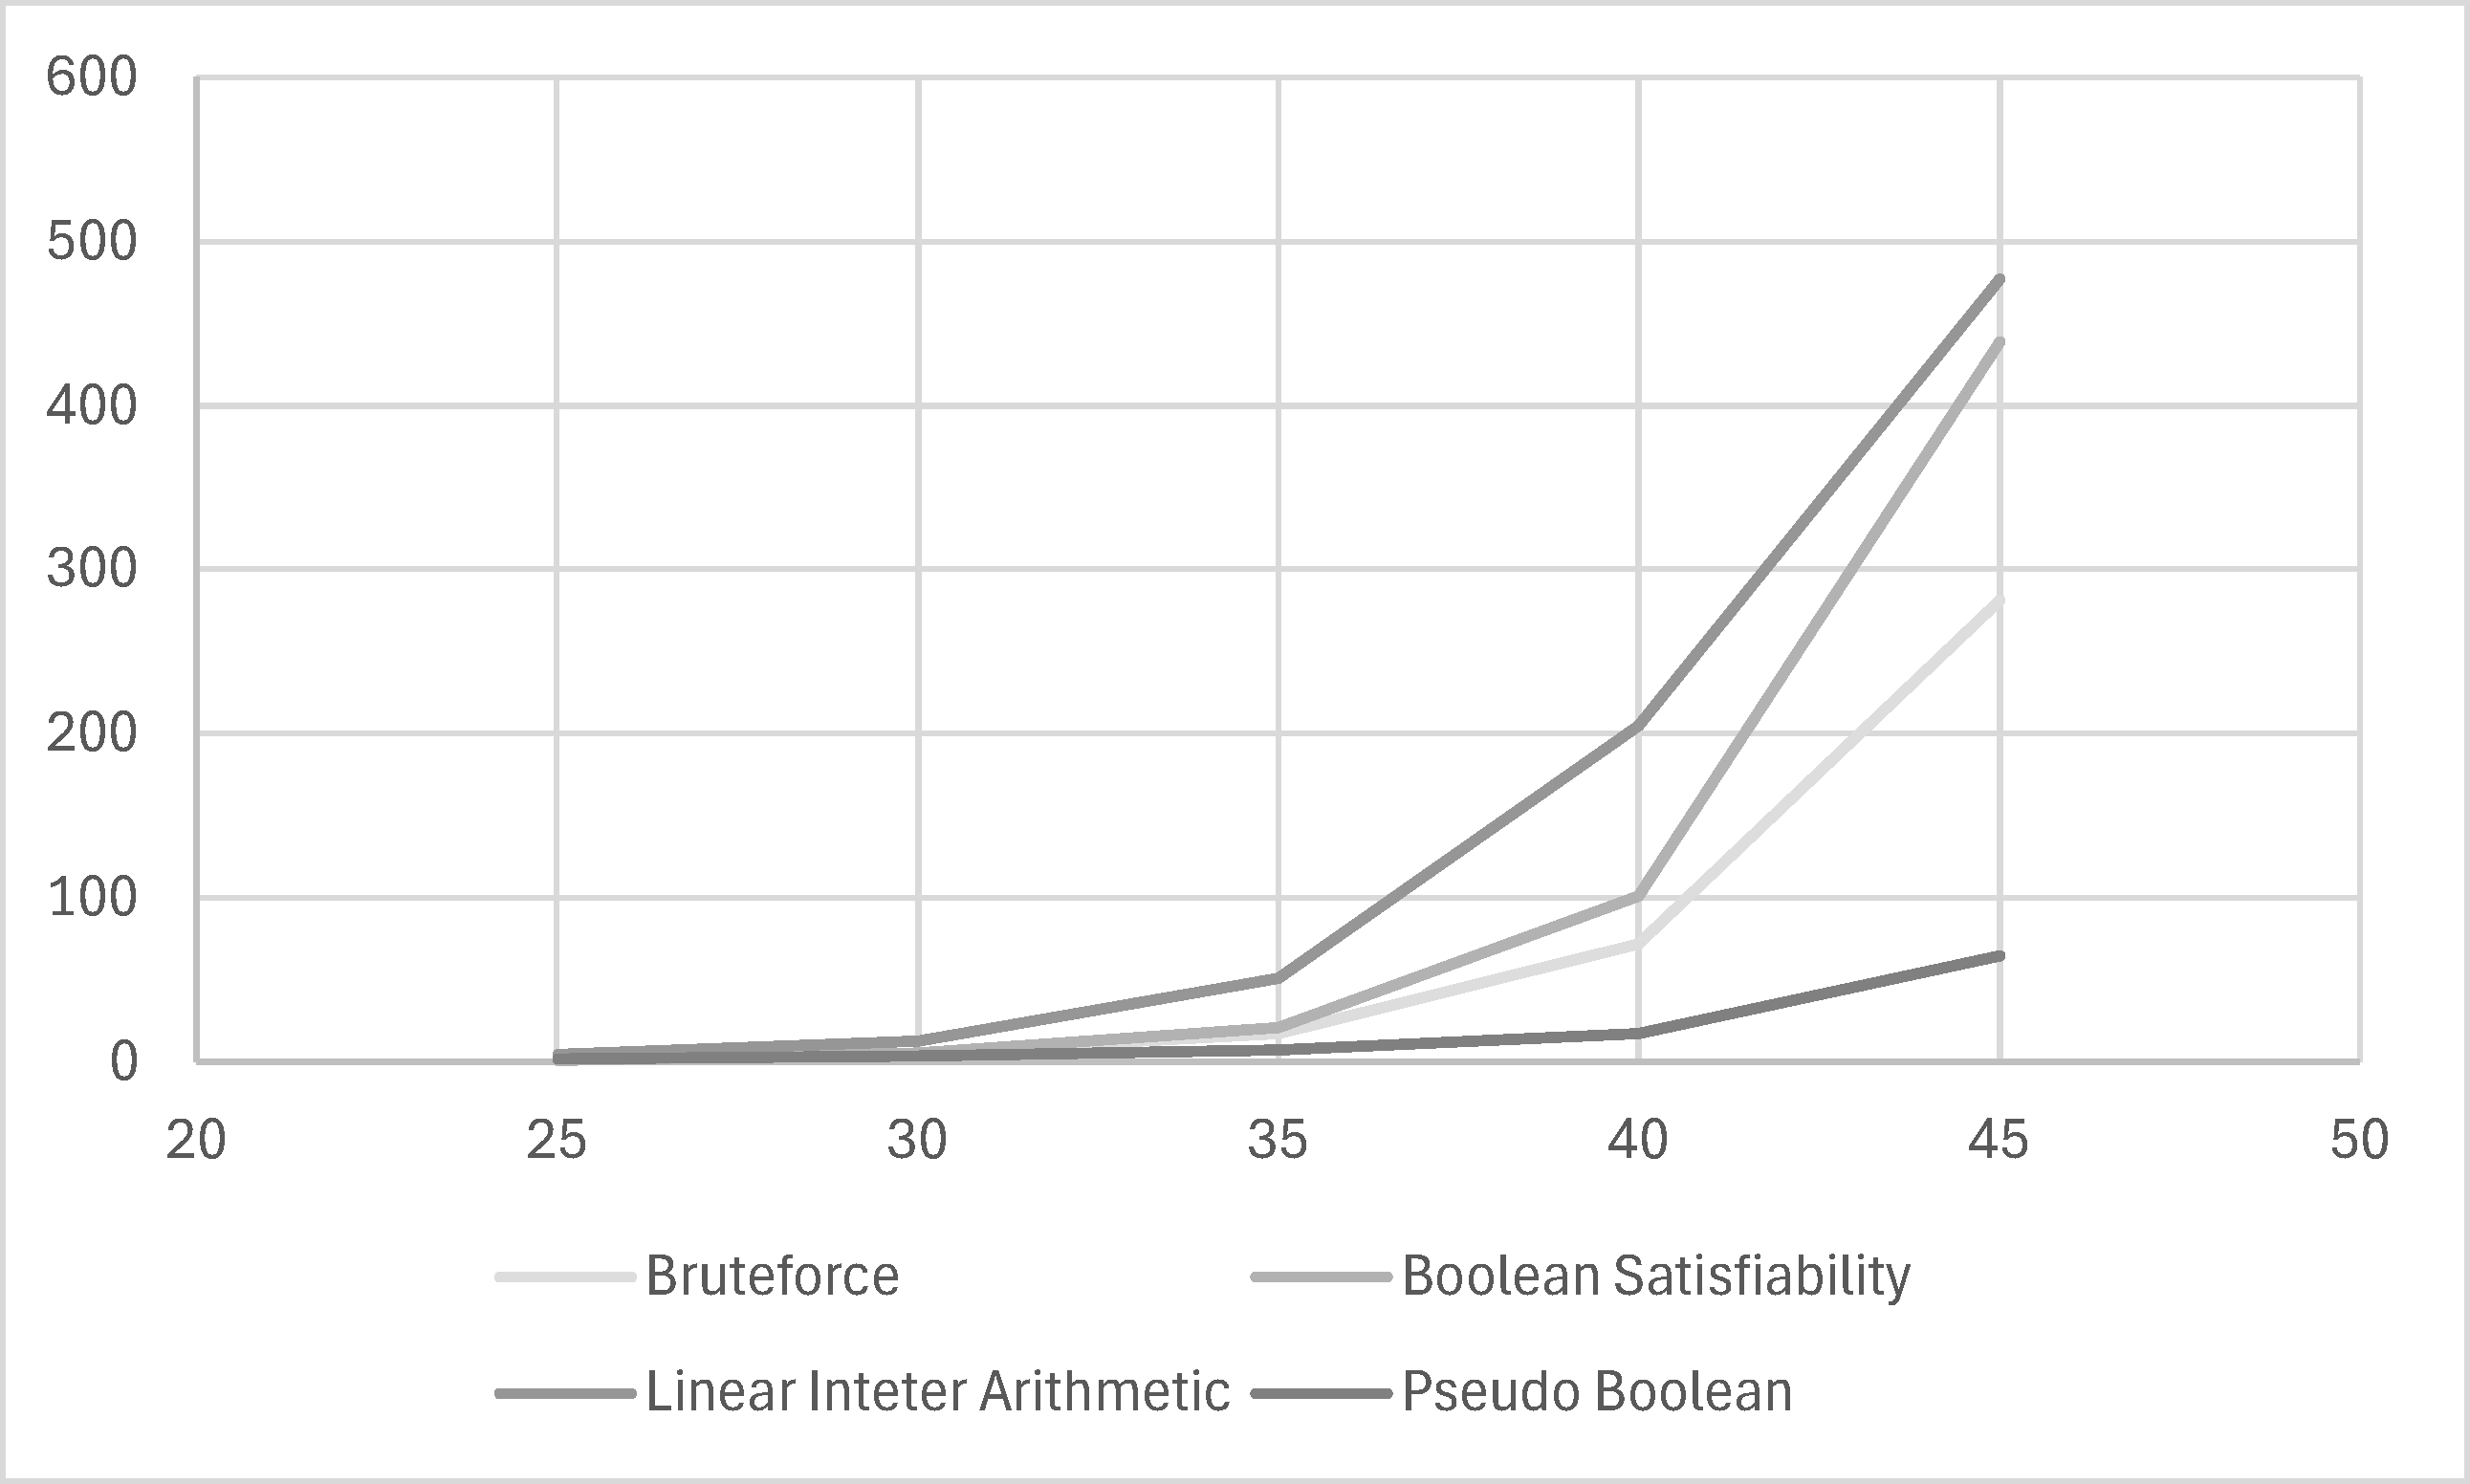
\includegraphics[width=\linewidth]{img/trend-md-large.pdf}

	Tren Waktu Eksekusi Dimensi Metrik Graf Besar
}{}

\slide{Tren Waktu untuk Graf Besar}{
	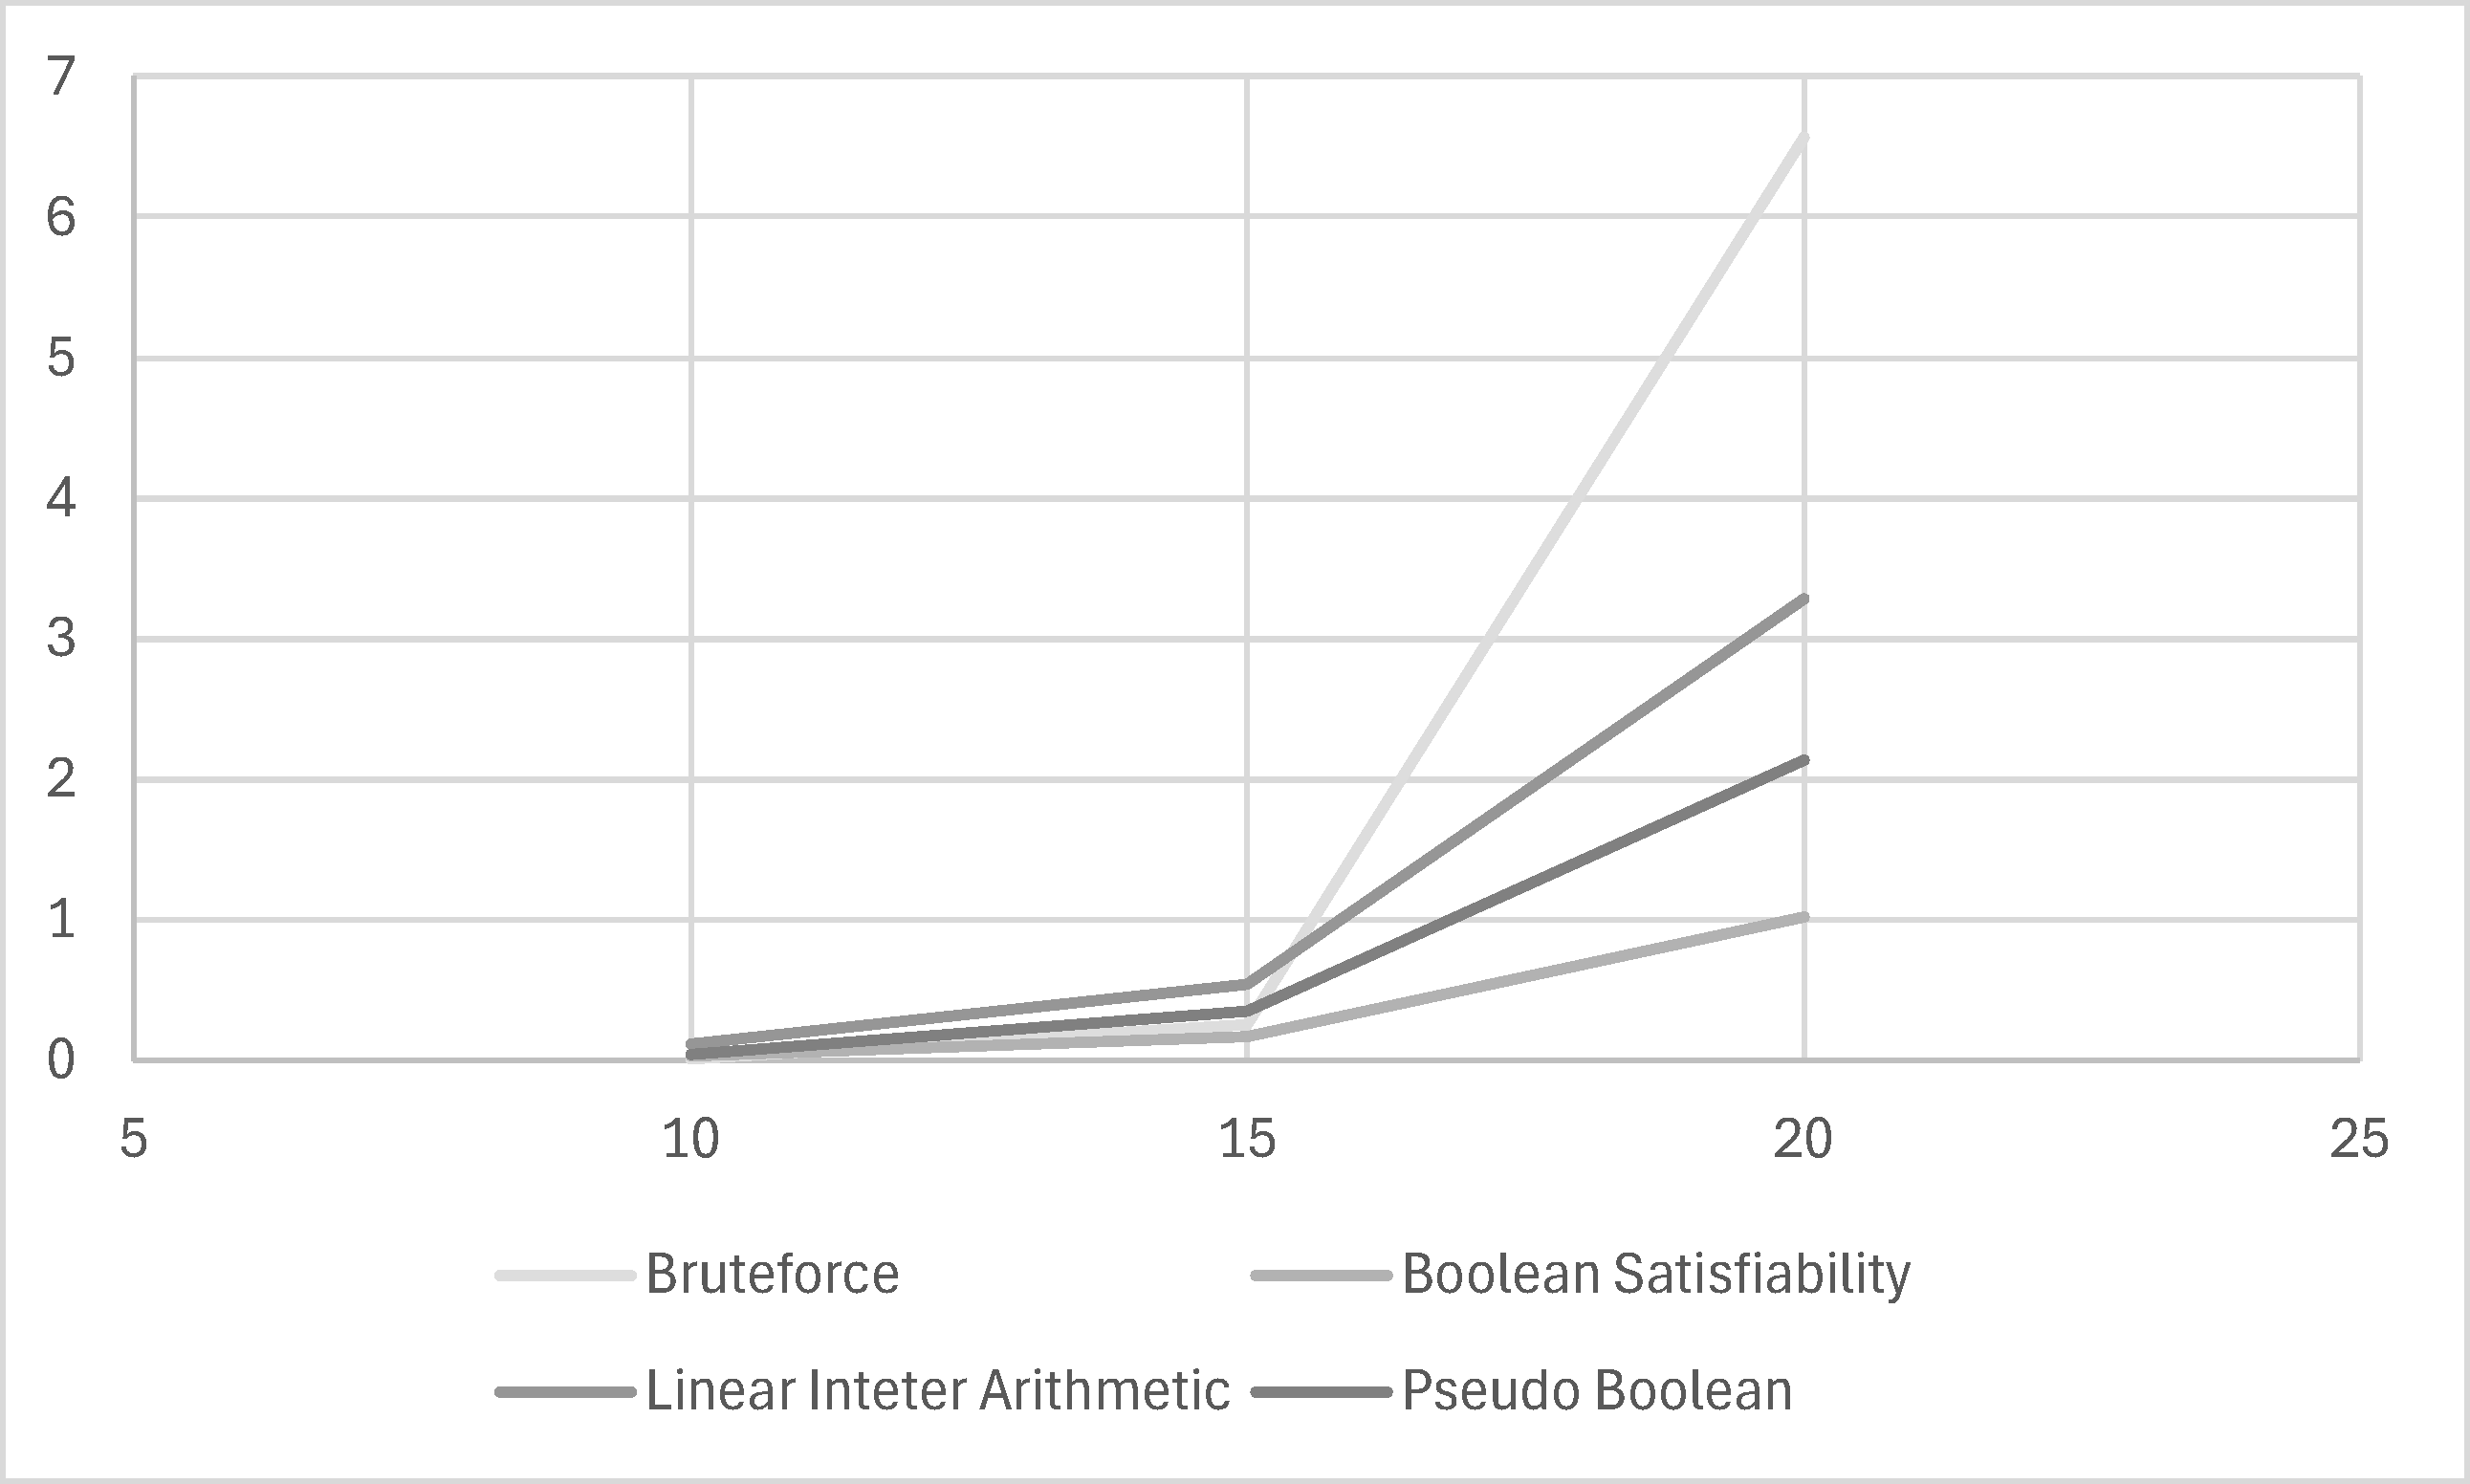
\includegraphics[height=52mm]{img/trend-emd-large-1.pdf}
	\hfill
	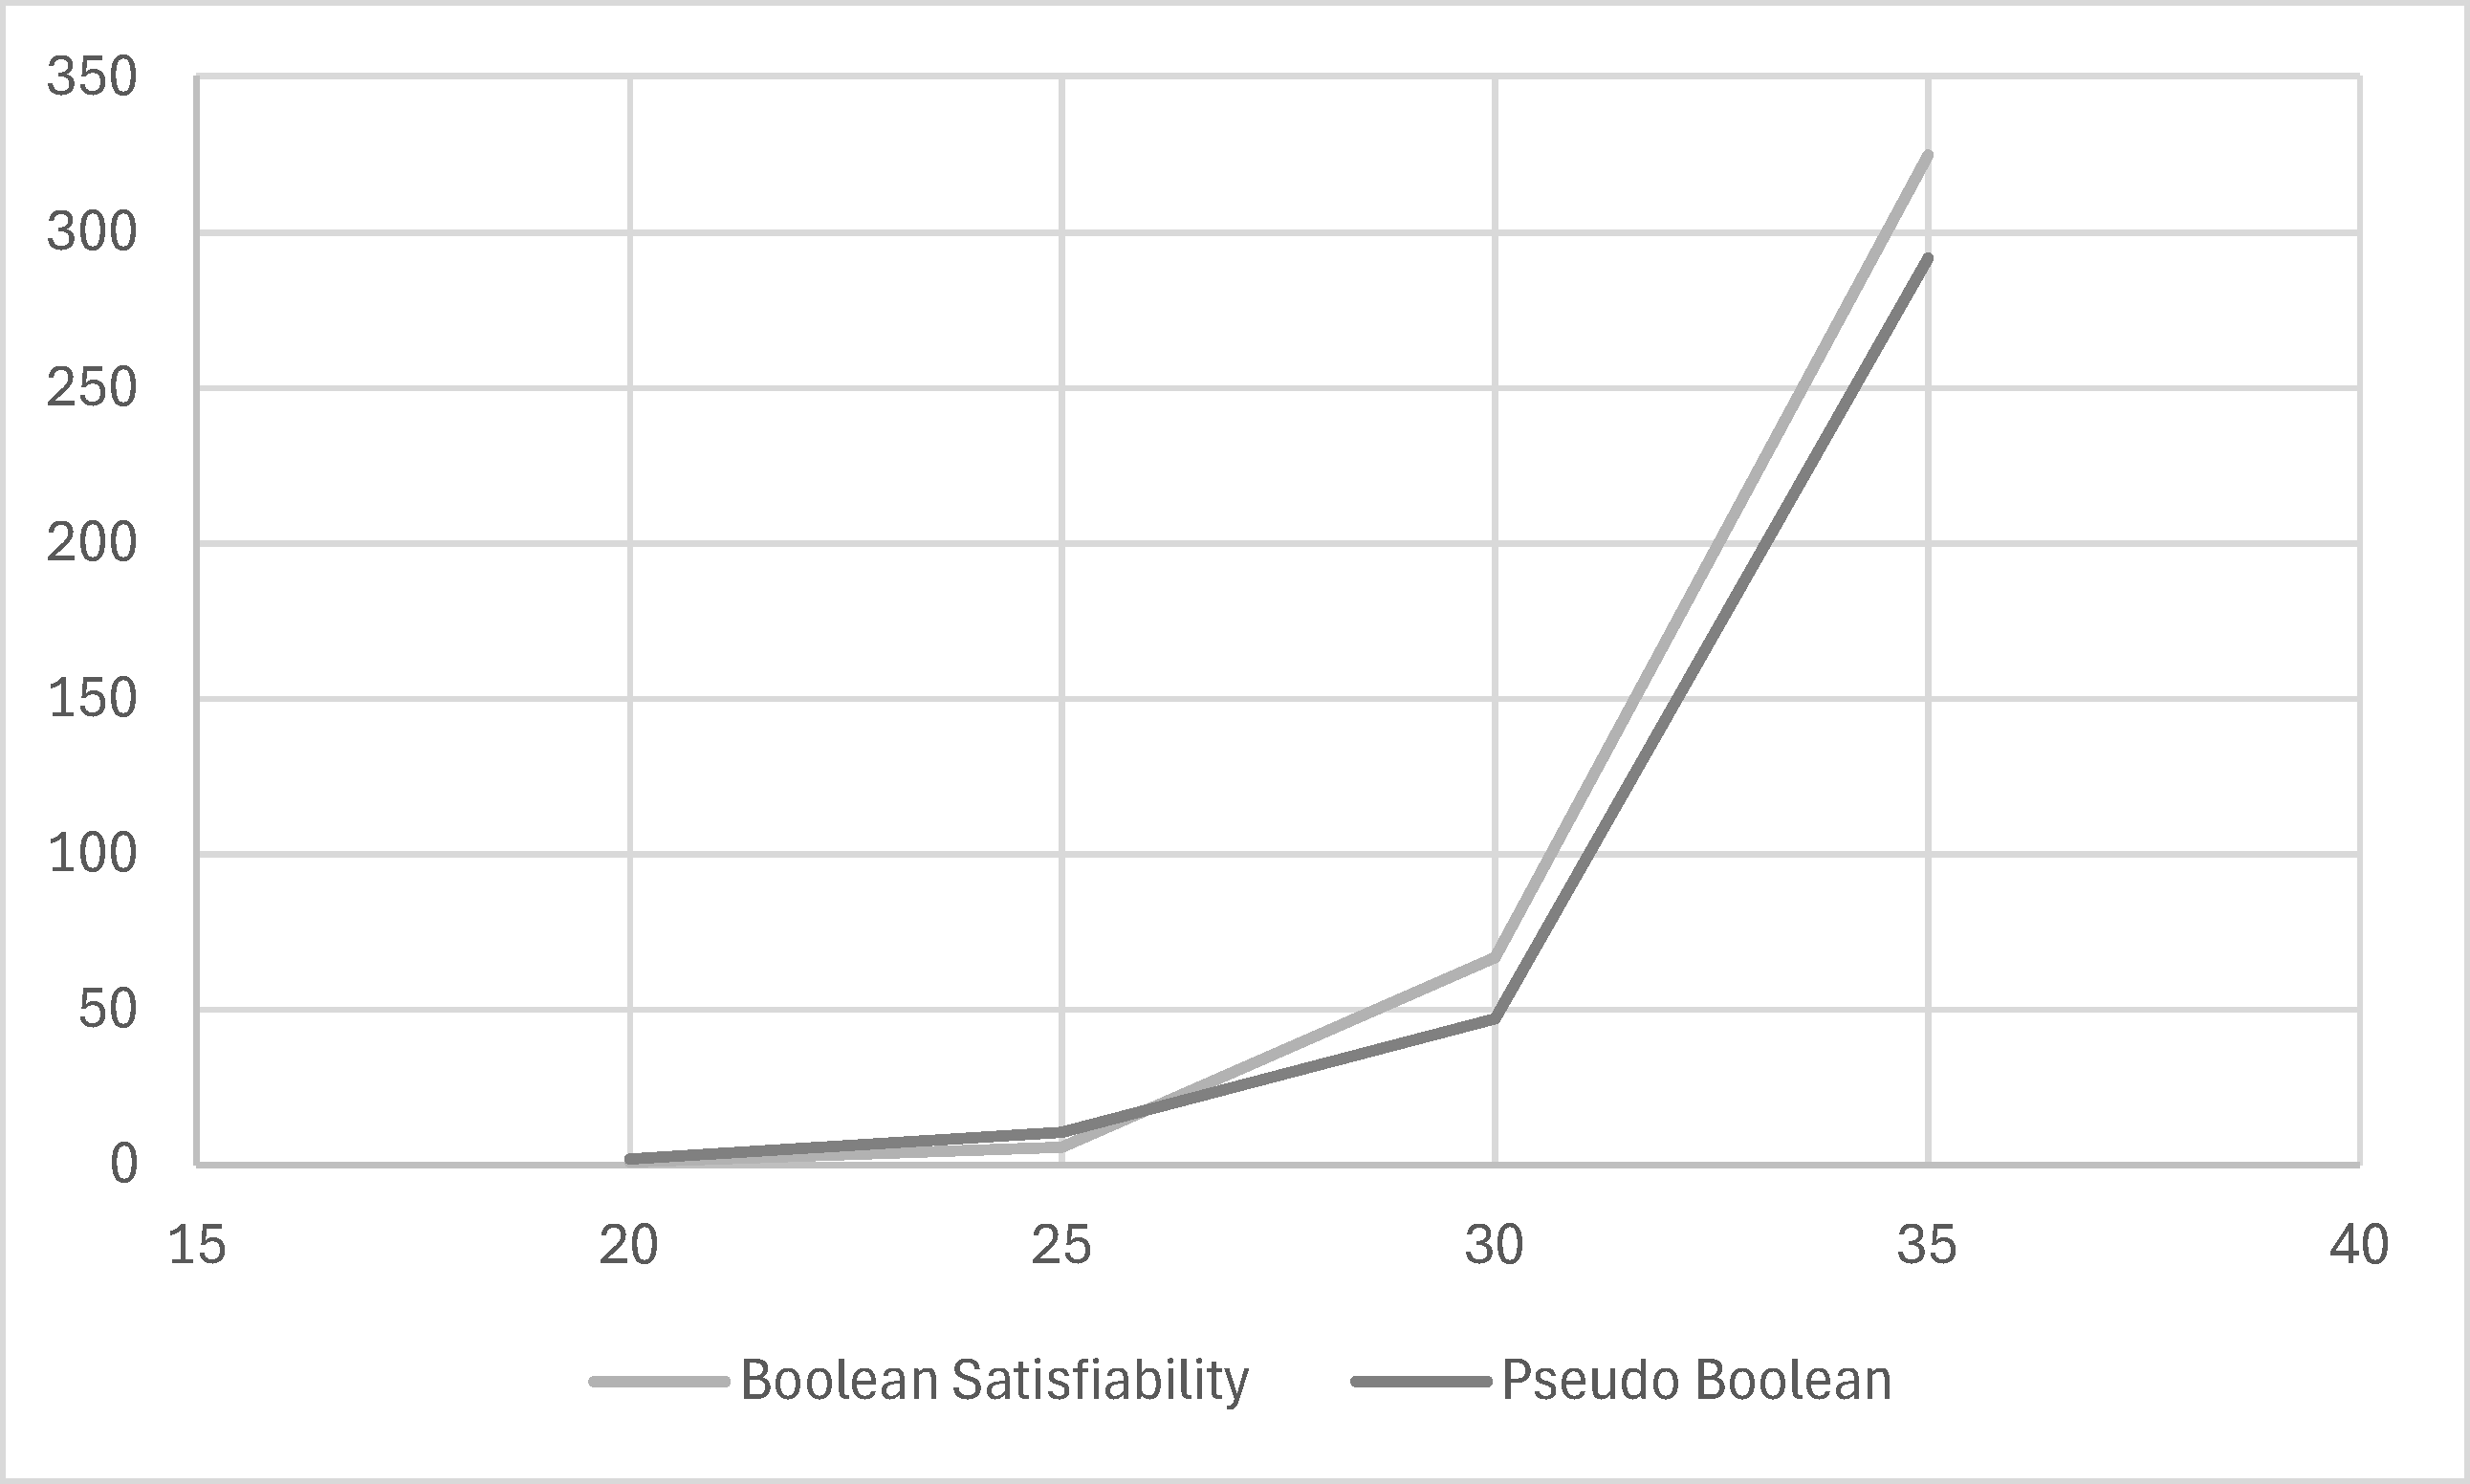
\includegraphics[height=52mm]{img/trend-emd-large-2.pdf}

	Tren Waktu Eksekusi Dimensi Metrik Sisi Graf Besar
}{}

\slide{Gambaran Besar Tren Waktu}{
	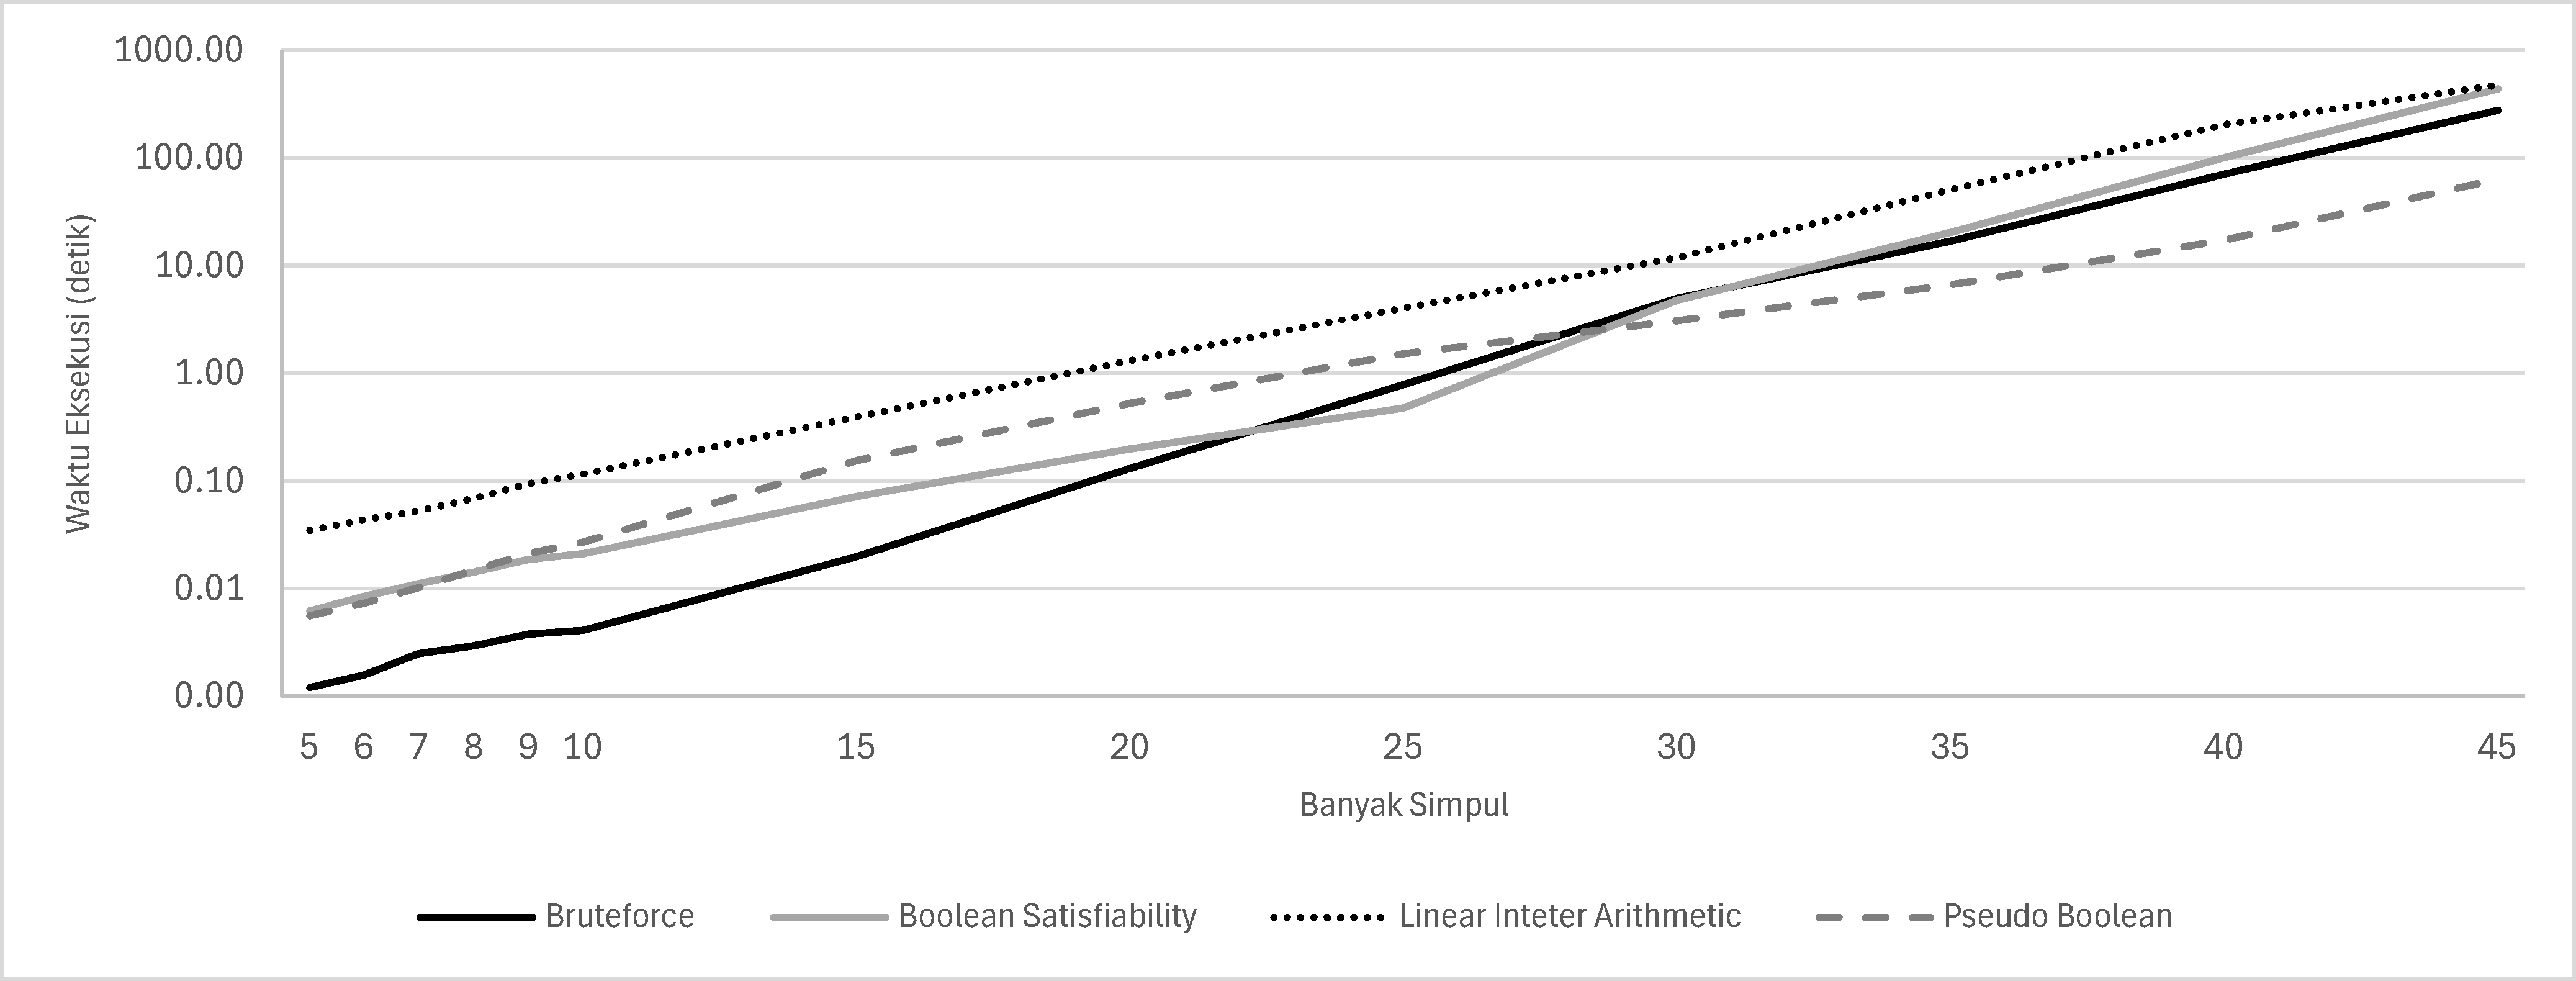
\includegraphics[width=\linewidth]{img/trend-md-combined.pdf}

	Tren Waktu Eksekusi Dimensi Metrik
}{}

\slide{Gambaran Besar Tren Waktu}{
	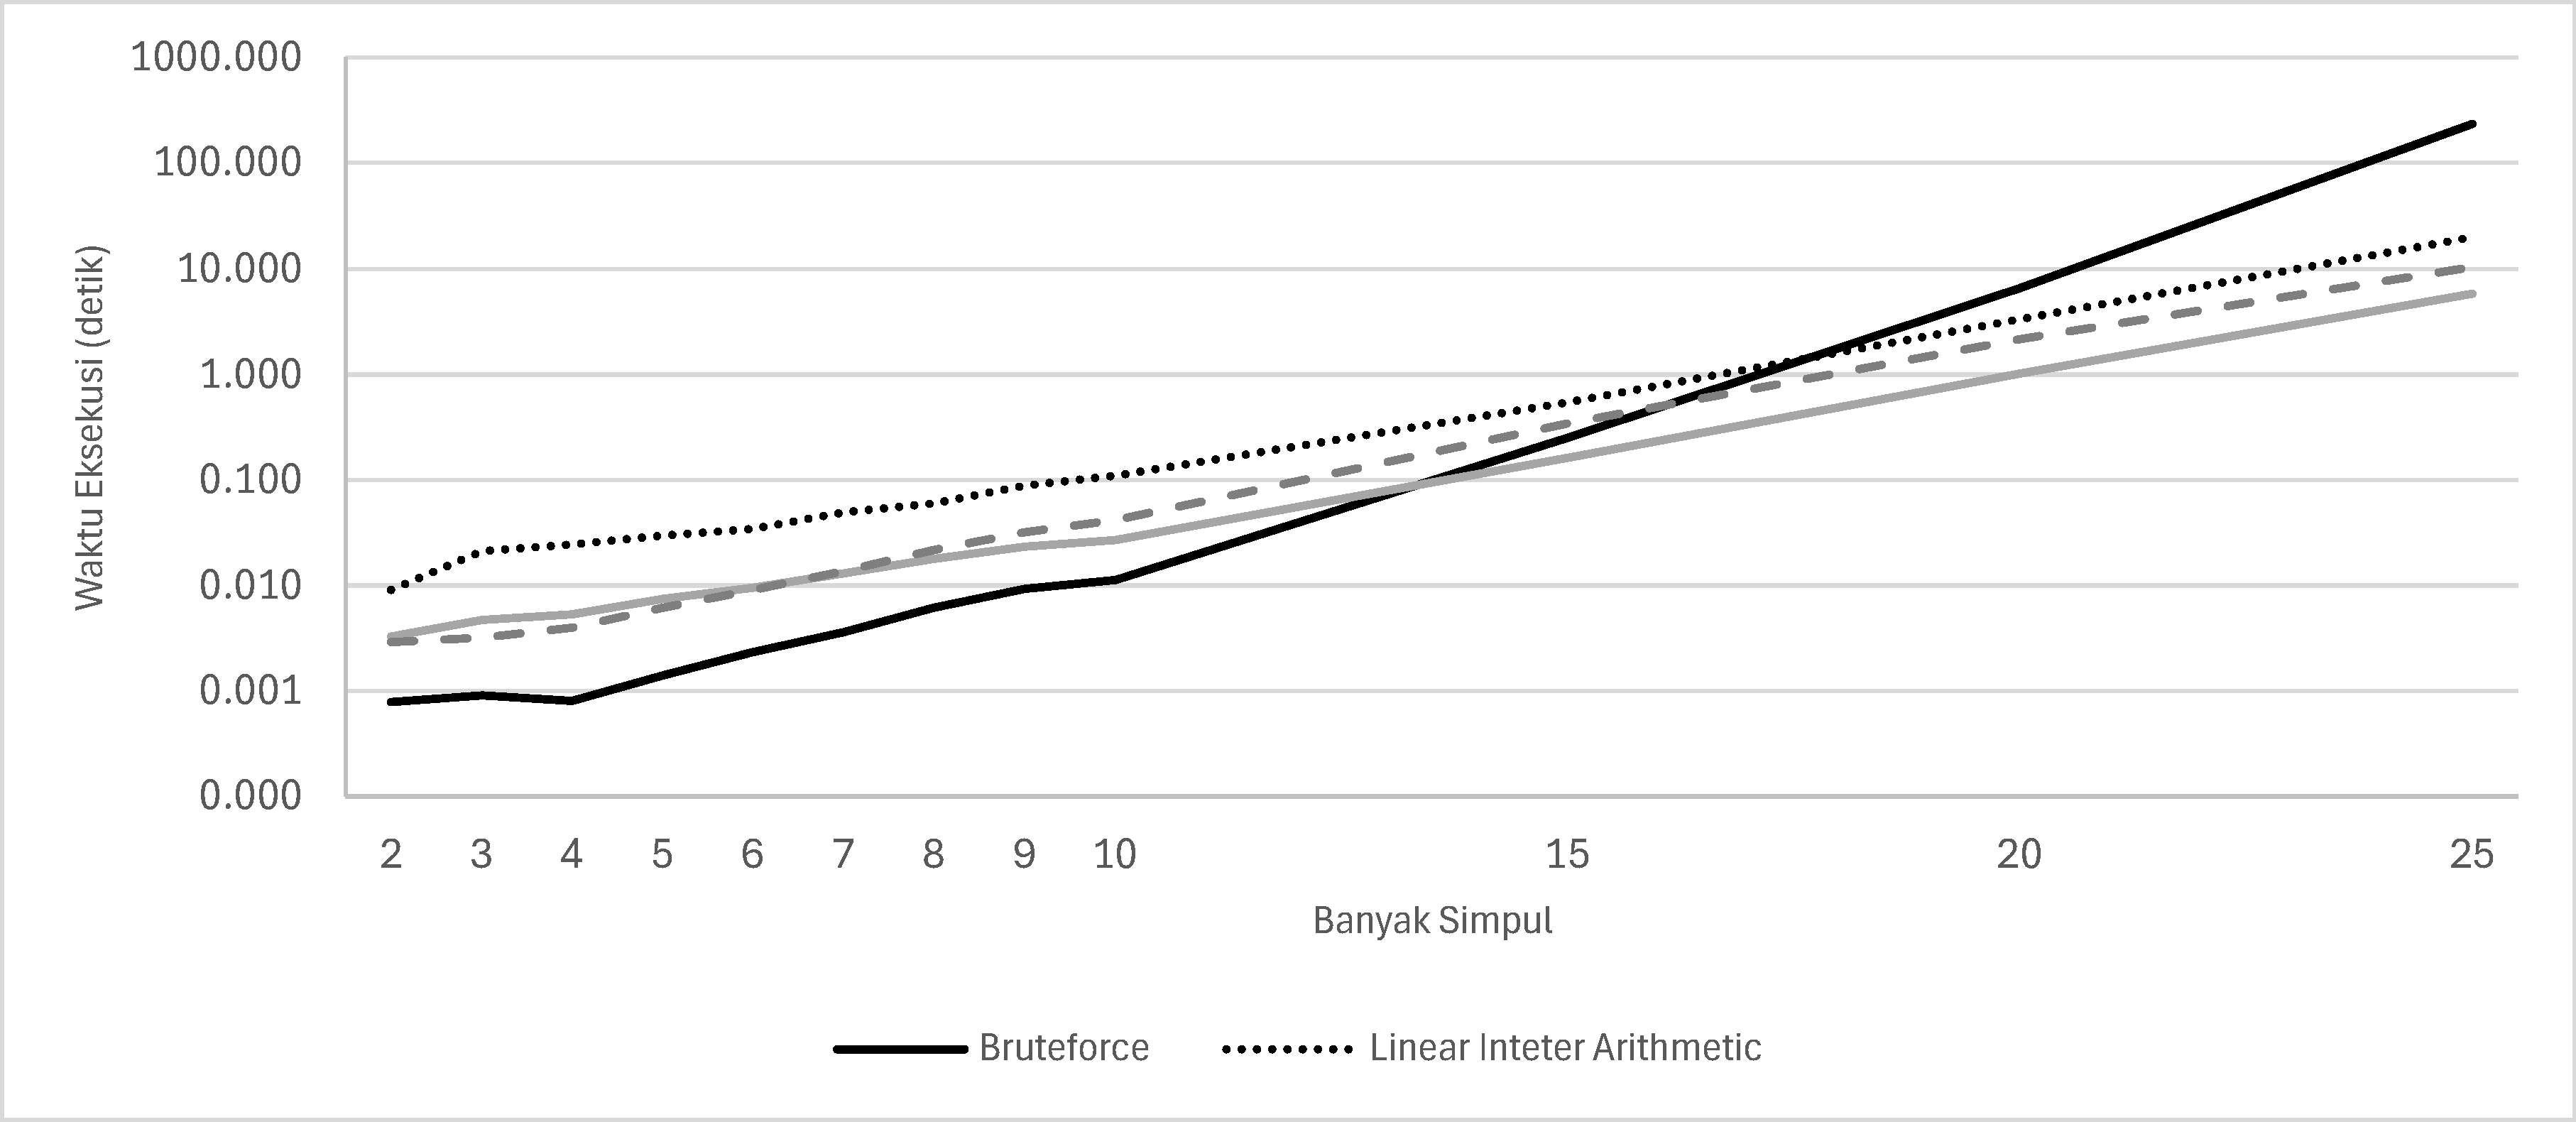
\includegraphics[height=41.5mm]{img/trend-emd-combined-1.pdf}
	\hfill
	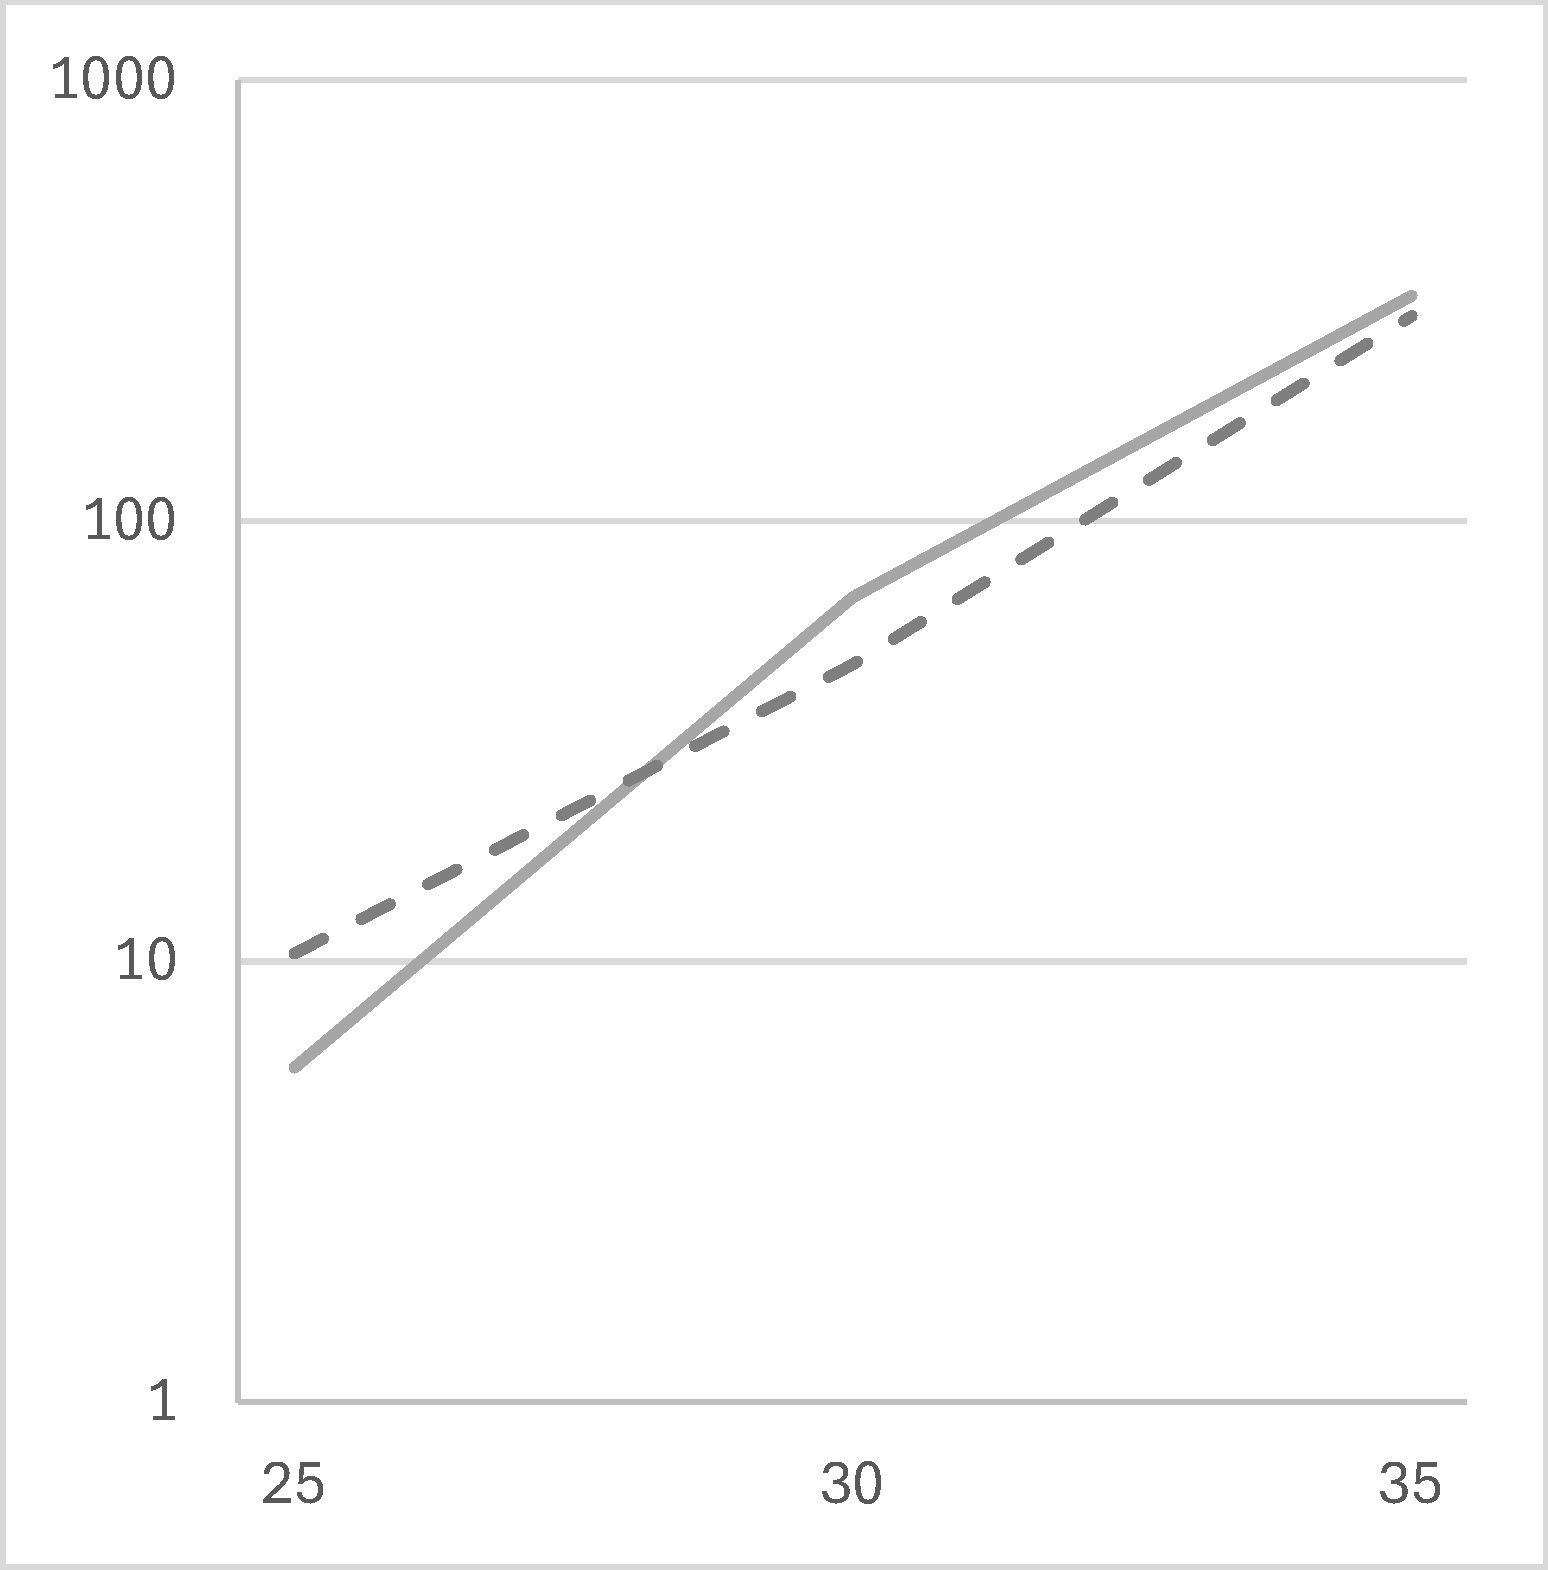
\includegraphics[height=41.5mm]{img/trend-emd-combined-2.pdf}

	Tren Waktu Eksekusi Dimensi Metrik Sisi
}{}

\outline{6}

\slide{Kesimpulan}{
	\begin{enumerate}
		\item Permasalahan dimensi metrik dapat direpresentasikan secara sistematis ke bentuk constraints SMT.

		\item Pendekatan SMT dapat digunakan secara praktikal untuk menentukan dimensi metrik suatu graf; bahwa strategi tersebut menghasilkan invarian ini dengan benar.

		\item Efektivitas penggunaan SMT dalam menyelesaikan permasalahan dimensi metrik bergantung pada ukuran graf dan sumber daya komputasi yang tersedia, serta pemilihan teori yang digunakan.
	\end{enumerate}
}{}

\titleslide{
	\textbf{\Large Terima Kasih}
}

\end{document}
